\documentclass[a4paper,10pt]{article}
\usepackage[utf8]{inputenc}
\usepackage{xspace}
\usepackage{url}
\usepackage{graphicx,graphics} 
\usepackage{color}
\usepackage{amsmath}
\usepackage{amsfonts}
\usepackage{amssymb}
\usepackage{amsthm}
\usepackage{algorithm}
\usepackage{algorithmic}
\usepackage{longtable}
\usepackage{complexity}
\usepackage{tkz-graph}
\usepackage{float}
\usepackage{setspace}
\renewcommand{\algorithmicrequire}{\textbf{Input:}}
\renewcommand{\algorithmicensure}{\textbf{Output:}}
\usepackage{authblk}
% \usepackage{hyperref}

\graphicspath{{figures/}}
\makeatletter
\def\input@path{{figures/}}
\makeatother
\newcommand\rmatching{${\cal R}$-matching\xspace}
\newcommand\mdelay{$\cal M$-delay\xspace}
\newcommand\matchedgraph{{\bf matched graph}}
\newtheorem{proposition}{Proposition}
\newtheorem{theorem}{Theorem}

\setlength{\parskip}{1ex} % Espace entre les paragraphes

\newtheorem{fact}{Fact}
\newtheorem{lemma}[theorem]{Lemma}
\newtheorem{definition}{Definition}
\newtheorem{corollary}{Corollary}

\renewcommand{\thefootnote}{\*}

\newcommand{\todo}[1]{{\color{red} TODO: {#1}}}


%opening
\title{Deterministic Scheduling of Periodic Messages in a Network}% by a SDN (deterministic) approach}


\author[1]{Ma\"el Guiraud}
\author[1]{Dominique Barth}
% \author[1]{Christian Cad\'er\'e}
\author[2]{Brice Leclerc}
\author[2]{Olivier Marc\'e}
\author[1]{Yann Strozecki}
\affil[1]{David Laboratory, UVSQ}
\affil[2]{Nokia Bell Labs France}

\begin{document}

\maketitle

\begin{abstract}
We study the sending of periodic messages in a graph following predefined paths, a problem arising from communication between radio antennas and their signal processing units located in distant data-centers. Messages must be sent deterministically to avoid collisions on the network and to minimize the latency. We prove that problems arising from this context are $\NP$-complete even for very restricted graphs. We then deal with the case of a star graph and for different regimes of the parameters we propose algorithms that are experimentally shown to work extremely well compared to traditional statistical multiplexing.
\end{abstract}

\footnote{This work is partially supported by the french ANR project N-GREEN.}
\section{Introduction}

Next generations of mobile network architectures evolve toward centralized radio network architectures called C-RAN, or Cloud Radio Access Network, to reduce energy consumption costs~\cite{mobile2011c} and more generally the total cost ownership. The main challenge for this type of architecture is the latency in the transfer process that is an important factor for dimensioning the network. The latency is measured between the sending of a message by the Remote Radio Heads (RRHs) on the field and the receptions of the answers, computed by real-time virtualized network functions on Baseband Units (BBUs), in the cloud. For example, even if next radio protocols are less stringent, some standards requires meeting time constraints for functions like HARQ (Hybrid Automatic Repeat reQuest) that needs to be processed in 1 to 10ms depending on targeted services~\cite{bouguen2012lte}. The specificity of the C-RAN context is not only the latency constraint, but also the periodicity of the data transfer between RRHs and BBUs.

 In this article, we study mechanisms to deal with the latency and periodicity constraints in the fronthaul network.  The current solution ~\cite{pizzinat2015things} is to use use dedicated circuits, since statistical multiplexing even with a very large bandwidth, does not comply with the latency requirements. 
 \todo{mettre la suite de l'Etat de l'art}
 Thus in this article, we work on latency and periodicity constraints in fronthaul. The best current solution is to rely on an almost full optical approach, where each end-point (RRH on one side, BBU on the other side) is connected through direct fiber or full optical switches ~\cite{tayq2017real}. This architecture is very expensive and hardly scales in the case of a mobile network composed of about 10,000 base stations. 
 
 
 Here we propose to use a deterministic approach to schedule our periodic messages. This approach has gained some traction recently: Deterministic Networking is under standardization in IEEE 802.1 TSN group~\cite{finn-detnet-architecture-08}, as well at IETF DetNet working group~\cite{ieee802}. Several patents on concepts and mechanisms for DetNet have been already published, see for example~\cite{howe2005time,leclerc2016transmission}. The aim is to operate a C-RAN on a low-cost shared switched network.
 
Let us expose briefly our model: the network topology is modeled by a directed weighted graph and a set of paths (routes) from source nodes (RRHs) to target nodes (BBUs). Time is discretized and a unit of time corresponds to the transmission of a minimal unit of data over the network. The process must be  predictable (i.e. the date of arrival of packets is known beforehand). For simplicity, in this article we assume that the process is periodic. That is, if we look at the network at times $t$ and $t+P$ where $P$ is the period, all messages are at the same position in the network. Moreover, we want to avoid any  buffering in internal nodes of the graph. Hence we need to design a periodic process with no collision between messages. To ensure that this property is always true we propose a deterministic process.  We have two sets of parameters that we can choose when building a periodic sending process, called a \textbf{periodic assignment} in this article: the time at which each packet is sent by a RRH in each period and the waiting time in the BBU before the answer is sent back to the RRH. When building a periodic assignment, we must take into account the periodicity which makes many scheduling methods inapplicable. Not only a message must not collide with the other messages sent by the others BBU/RRH in the same period, but also in the previous and following periods. Moreover the latency must be minimized, that is the time 
 between the emission of a message and the complete return of its answer. It means that the only buffering we are allowed -- the waiting time before sending back the answer-- must be small, in particular when the route is long.
 

 
%  Hence a solution is needed to offer low latency over commoditized packet based networks. Indeed, dynamical optical bypass and dynamical management of the emission should be considered to guarantee latency constraints, as in the french ANR project N-GREEN. This project proposes a new type of switching/routing node and a specific network architecture exploiting WDM packets thanks to a new generation of optical add/drop multiplexers (WSADM: WDM slotted add/drop multiplexer). These packets having a fixed duration close to 1?s are transported in a transparent way, to better exploit the switching matrix of the node; their headers will be transported over one dedicated wavelength at a lower bit rate, to reduce the physical constraints of the electronic processing and scheduler. 
%  
The problem we focus on here may look like wormhole problems~\cite{cole1996benefit}, but here we want to minimize the time lost in buffers and not just to avoid deadlocks, moreover the periodicity is not considered in wormhole problems. Several graph colorings have been introduced to model similar problems such as the allocation of frequencies~\cite{borndorfer1998frequency}, bandwidths~\cite{erlebach2001complexity} or routes~\cite{cole1996benefit} in a network or train schedules~\cite{strotmann2007railway}. Unfortunately, they do not take into account the periodicity of the scheduling and the associated problems are already $\NP$-complete. The only model which incorporates some periodicity is the circular coloring~\cite{zhou2013multiple, zhu2001circular,zhu2006recent} but is not expressive enough to capture our problem.


 In Sec.~\ref{sec:def} we propose a model of the network and the periodic sending of messages along its routes. 
 We then formalize our two problems of finding a periodic assignment for sending messages without collisions: PRA (sending of the message only) and PALL (sending of the message and of the answer).  
In Sec.~\ref{sec:complexity}, we prove that the problem PRA and PALL are $\NP$-hard and cannot be approximated even for very
restricted classes of graphs. 
Therefore in the next two sections, we study a simple but very common topology, that we call the
star topology, where all messages can collide on a single arc.
In Sec.\ref{sec:PAZL}, we study a variant of PALL called PAZL  where the waiting times must all be zero. We provide several algorithms, some of their theoretical properties and give experimental evidences that they find periodic assignments when the network is not too loaded. Finally in Sec.\ref{sec:PALL}, we propose algorithms for the general PALL problem and exhibit one which works extremely well in our experiments even in loaded networks. In particular we show that the deterministic communication schemes we design vastly outperform the traditional stochastic multiplexing with regard to latency. 


\section{Model and Problems}\label{sec:def}

  \subsection{Network modeling}
  

The network is modeled as a directed graph $G=(V,A)$. Each arc  $(u,v)$ in $A$ is labeled by an integer weight $\omega(u,v)$ which represents the time slots taken by a signal to go from $u$ to $v$ using this arc. A {\bf route} $r$ in $G$ is a path, that is sequence of consecutive arcs $a_0, \ldots , a_{k-1}$, with $a_i=(u_i,u_{i+1}) \in A$.  The {\bf latency} of a vertex $u_i$ in a path $r$, with $i \geq 1$, is defined by $\lambda(u_i,r)= \sum\limits_{0 \leq j <i} \omega(a_j)$. We also define $\lambda(u_0,r)=0$. The length of the route $r$ is defined by $\lambda (r)= \lambda (u_k,r)$.
We denote by $\cal R$ a set of routes,  %in $G$ such that no two routes have the same first vertices or the same last vertices.
the pair $(G,\cal R)$ is called a {\bf routed network} and represents our telecommunication network.
The first vertex of a route models an antenna (RRH) and the last one a data-center (BBU) which processes the messages sent by the antenna.

%We denote by $\rho$ the bijection induced by ${\cal R}$, $\rho(s) = t$ if $s$ is the first vertex of a route $r$ and $t$ the last. 



   \subsection{Messages dynamic}
      
      Consider a route $r$, if a message is sent at time $m$ from $s$ the first vertex of $r$ then it will arrive at vertex $v$ in $r$ at time $m + \lambda(v,r)$. In our problem, we send one message on each route periodically and we denote the period by $P$.
      Periodicity means that if we look at the messages going through an edge between time $0$ and $P-1$, then we would observe the same messages in the same order and position between time $kP$ and $(k+1)P -1$ for all $k$. 
      Therefore, we will always consider a period of $P$ discrete slots of time at each edge to characterize the working of the network. We define the first time slot at which a message sent from the first vertex of $r$ will reach a vertex $v$ in $r$ by $t(v,r) = m + \lambda(v,r) \mod P$. 
      
      A message usually cannot be transported in a single time slot. We denote by $\tau$ the number 
      of \emph{consecutive slots} necessary to transmit a message. Let us call $[t(v,r)]_{P,\tau}$ the set of time slots used by route $r$ at vertex $v$ in a period $P$, that is $[t(v,r)]_{P,\tau} = \{t(v,r) + k \mod P \mid 0 \leq k < \tau \}$. Usually $P$ and $\tau$ will be clear from the context and we will denote $[t(v,r)]_{P,\tau}$ by $[t(v,r)]$.
      Let $r_1$ and $r_2$ be two routes, on which messages are sent at time $m_1$ and $m_2$ in their first vertex.
      We say that the two routes have a {\bf collision} if they share an arc of first vertex $v$ and $[t(v,r_{1})] \cap [t(v,r_{2})] \neq \emptyset$.
      
      \todo{commencer les routes  0 ou pas ?}
      
      A {\bf $(P,\tau)$-periodic assignment} of a routed network $(G,\cal R)$ is a sequence  ${\cal M}=(m_0, \ldots ,m_{n-1})$ of $n$ integers that we call {\bf offsets}, with $n$ the number of routes in $\cal R$. The number $m_{i}$ represents the time at which a message is emitted at the first vertex of the route $r_{i}$. We will always consider that the $m_{i}$ are between $0$ and $P-1$. Moreover, \emph{no pair of routes must have a collision} in a $(P,\tau)$-periodic assignment.
      

%       Notice that the notion of $P$-periodic assignment \textbf{is not monotone} with regard to $P$. 
      As an example of a $(2,1)$-periodic assignment, let us consider a routed network 
      where all pairs of routes intersect at a different edge. It is easy to design such a network and an example is given in Fig.~\ref{fig:example}. We set $\tau = 1$ and the weights are chosen so that if $r_{i}$ and $r_{j}$ have $v$ as first common vertex then we have $\lambda(v,r_{i}) - \lambda(v,r_{j})=1$. There is a $(2,1)$-periodic assignment by setting all $m_{i}$ to $0$.

  
      \begin{figure}[ht]
      \begin{center}
          \scalebox{0.8}{
          
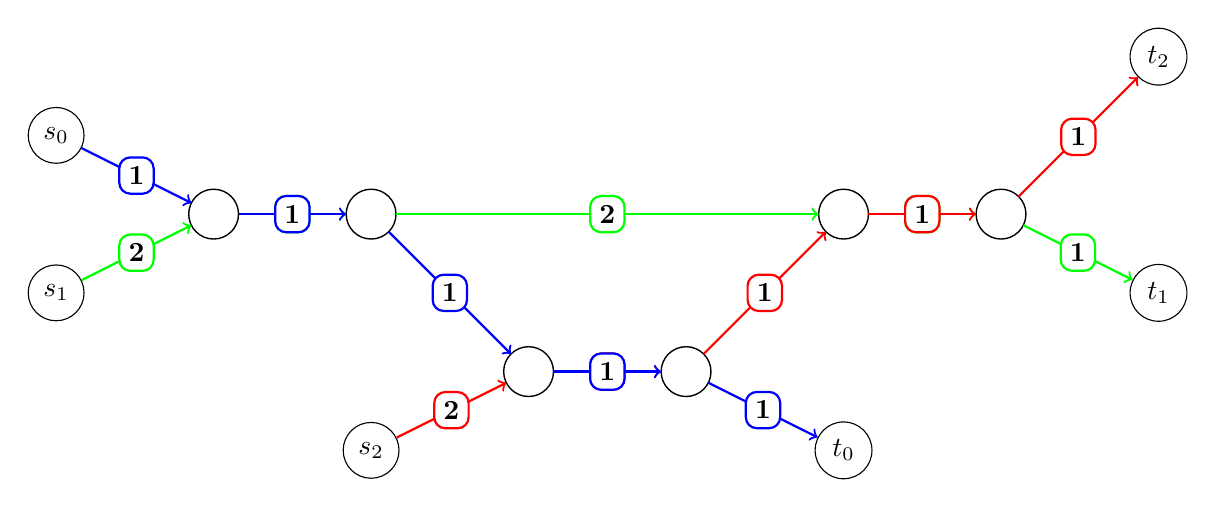
\begin{tikzpicture}


\tikzset{
  LabelStyle/.style = { rectangle, rounded corners, draw,
                       font = \bfseries },
  EdgeStyle/.append style = {->} }
  \SetGraphUnit{5}
  \node[draw,circle] (s3) at (4, 2) {$s_2$}; 
  \node[draw,circle] (s2) at (0, 4) {$s_1$}; 
  \node[draw,circle] (s1) at (0, 6) {$s_0$}; 

  \node[draw,circle] (t3) at (14, 7) {$t_2$}; 
  \node[draw,circle] (t2) at (14, 4) {$t_1$}; 
  \node[draw,circle] (t1) at (10, 2) {$t_0$}; 

  
  \SetVertexNoLabel
  \Vertex[x=2,y=5]{A}
  \Vertex[x=4,y=5]{B}
  \Vertex[x=10,y=5]{C}
  \Vertex[x=12,y=5]{D}
  \Vertex[x=6,y=3]{E}
  \Vertex[x=8,y=3]{F}
  \tikzset{
  EdgeStyle/.append style = {green} }
  \Edge[label = 2](s2)(A)
  \Edge[label = 1](A)(B)
  \Edge[label = 2](B)(C)
  \Edge[label = 1](C)(D)
  \Edge[label = 1](D)(t2)

  
   \tikzset{
  EdgeStyle/.append style = {red} }
  \Edge[label = 2](s3)(E)
  \Edge[label = 1](E)(F)
  \Edge[label = 1](F)(C)
  \Edge[label = 1](C)(D)
  \Edge[label = 1](D)(t3) 
     \tikzset{
  EdgeStyle/.append style = {blue} }
  \Edge[label = 1](s1)(A)
  \Edge[label = 1](A)(B)
  \Edge[label = 1](B)(E)
  \Edge[label = 1](E)(F)
  \Edge[label = 1](F)(t1)

\end{tikzpicture}

}
     \end{center}
       \caption{A routed network with $(0,0,0)$ as a $(2,1)$-periodic assignment}
       \label{fig:example}
      \end{figure}

      \subsection{Periodic route assignment}\label{nonmonotone}

    We want to find an assignment which allows to send periodic messages from sources to targets
    without collisions. We introduce the following associated decision problem, useful for hardness proofs.
    

      \noindent {\bf  Periodic Routes Assignment (PRA)} 

      \noindent {\bf Input:} a routed network $(G,\cal R)$, an integer $\tau$ and an integer $P$.

      \noindent {\bf Question:} does there exist a $(P,\tau)$-periodic assignment of $(G,\cal R)$ ?


      We will prove in Sec.~\ref{sec:complexity} that the problem PRA is $\NP$-complete, even in restricted settings.
      In fact, approximating the smallest value of $P$ for which there is a $(P,\tau)$-periodic assignment is already hard.
      
      An unusual property of assignment is that given a routed network, we may have a $(P,\tau)$-periodic assignment but no
      $(P',\tau)$-periodic assignment with $P' > P$: the existence of an assignment is not monotone with regard to $P$.

	\begin{lemma} \label{lemma:monotonic}
	 For any odd $P$, there is a routed network such that there is $(2,1)$-periodic assignment but no $(P,1)$-periodic assignment.
	\end{lemma}
\begin{proof}

      Consider the routed network $(G,{\cal R})$ given in the previous subsection. 
      We change the weights so that for $v$, the first vertex which belongs to $r_i$ and $r_j$,
      we have $\lambda(v,r_i) - \lambda(v,r_j)= P$, where $P$ is an odd number smaller than $n$, the number of routes in ${\cal R_{\cal C}}$. In such a graph, there is no $(P,\tau)$-periodic assignment, since the problem reduces to finding a $P$-coloring in a complete graph with $n > P$ vertices, the colors beings the offsets of the routes.\\
      If we consider a period of $2$, for all $i \neq j$, $\lambda(v,r_i) - \lambda(v,r_j) \mod 2 = 1$ . Therefore $(0,\dots,0)$ is a $(2,1)$-periodic assignment of ${\cal R}$.      
\end{proof}
      
      
      \subsection{Periodic assignment for low latency}
      In the context of cloud-RAN applications, we need to send message from a RRH $u$ to a BBU $v$ and then 
      we must send the answer from $v$ back to $u$. We say that a routed network $(G, {\cal R})$ is \textbf{symmetric} if the set of routes is partitioned into the sets $F$ of forward routes and $B$ of backward routes. Moreover there is a bijection $\rho$ between $F$ and $B$ such that for any forward route $r \in F$ with first vertex $u$ and last vertex $v$, the backward route $\rho(r) \in B$ has first vertex $v$ and last vertex $u$. In all practical cases the routes $r$ and $\rho(r)$ will be the same with the orientation of the arcs reversed, which corresponds to bidirectional links in the networks, but we need not to enforce this property.
         
         We now give a new interpretation of a $(P,\tau)$-periodic assignment of a $(G,{\cal R})$ symmetric routed network, so that it represents the sending of a message and of its answer.
	This assignment represents the following process: first a message is sent at $u$, through the route $r \in F$, at time $m_r$.
       
      
      
      \begin{center}
      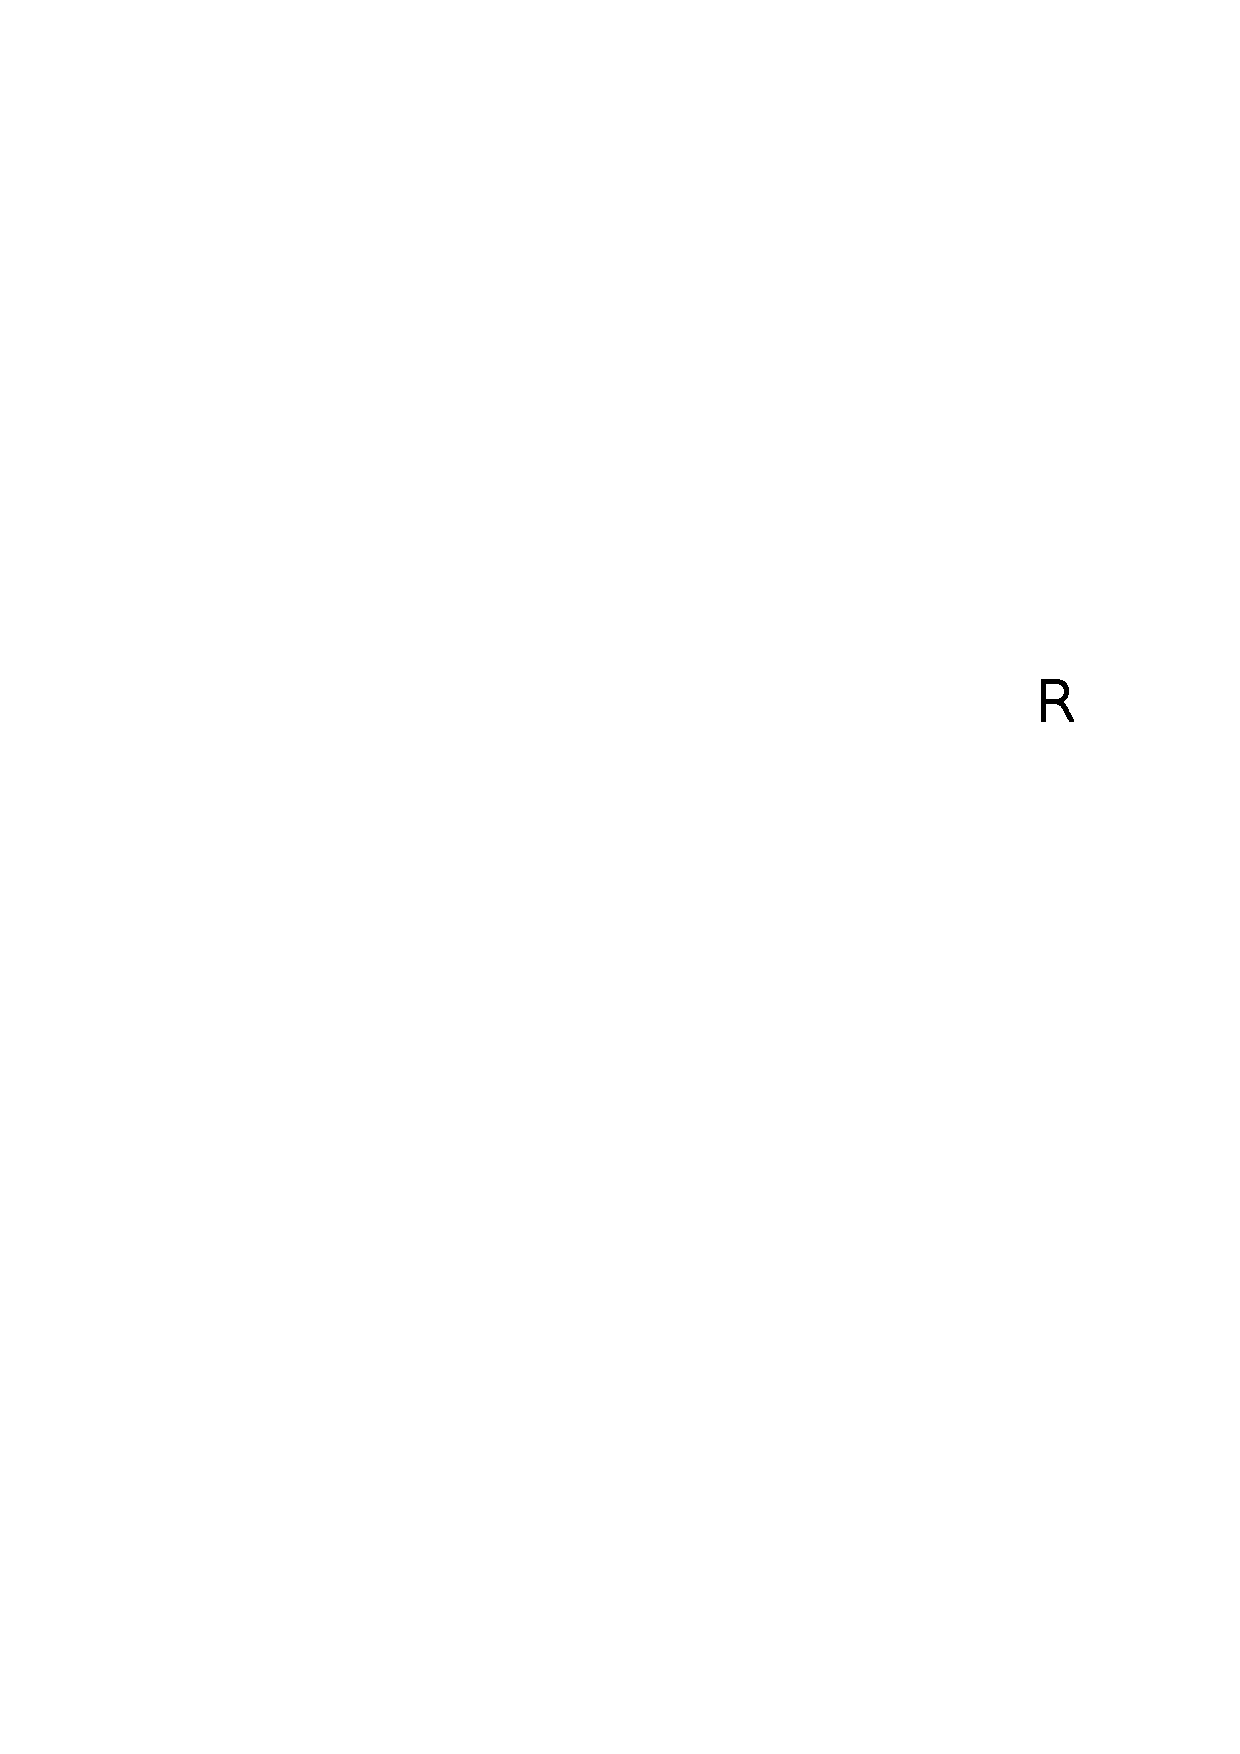
\includegraphics[width=\textwidth]{rrh.pdf}
      \end{center}
      
      

      This message is received by $v$ the last vertex of $r$ at time $t(v,r)$. It is then sent back to $u$ on the route $\rho(r)$ in the same period at time $m_{\rho(r)}$ if $m_{\rho(r)} > t(v,r)$, otherwise at time $m_{\rho(r)}$ in the next period. The time between the arrival of the message and the time it is sent back is called the \textbf{waiting time} and is defined by $w_r = m_{\rho(r)} - t(v,r)$ if $m_{\rho(r)} > t(v,r)$ and $w_r = m_{\rho(r)} + P - t(v,r)$ otherwise.
 
       \begin{center}
      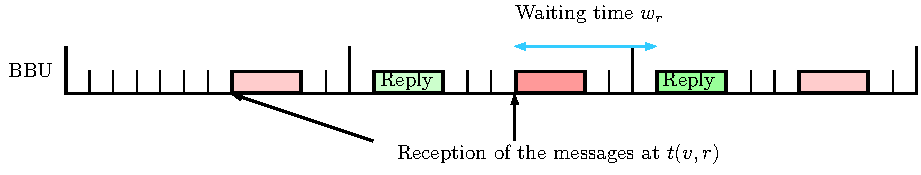
\includegraphics[width=\textwidth]{BBU.pdf}
      \end{center}
     
    
      Thus, the whole process time for a message sent on the route $r$ is equal to
      $PT(r)=\lambda(r)+ w_r+\lambda(r)$.      
      In the process time, we count the time between the first time at which a message is emitted and the first time at which the message comes back. Alternatively we could consider the time between the emission of the first slot and the reception of the last slot of the message, which would add $\tau$ to the process time.
      However, since all messages are of size $\tau$, it will not change the problems we consider in the rest of the article.
      Finally, we could add to the process time the computation time a BBU needs to deal with one message, but it can be encoded  in the weight of the last arc leading to the BBU and thus we need not to consider it explicitly in our model.
      
      
    The {\bf maximum process time} of the assignment ${\cal M}$ of $(G,{\cal R})$ is defined by $MT({\cal M})=\max\limits_{r \in {\cal R}} PT(r)$. We consider the following decision problem.

      \noindent {\bf Periodic Assignment for Low Latency (PALL)} 

      \noindent {\bf Input:}  A symmetric routed network $(G,{\cal R})$, the integers $P$, $\tau$ and $T_{max}$.

      \noindent {\bf Question:} does there exist a $(P,\tau)$-periodic assignment ${\cal M}$ of $(G,{\cal R})$ such that $MT({\cal M}) \leq T_{max}$?

      As a consequence of the $\NP$-hardness of PRA, we show in the next subsection that this problem is $\NP$-hard. 
      In Sec.~\ref{sec:PALL} we will study heuristics which try to solve the search version of PALL (computing an assignment), also denoted by PALL for simplicity.

     
      The following table summarize the main notations used in the paper.
      \begin{center}
   \begin{tabular}{|c|c|}
    \hline
     $(G,\cal R)$ & Routed network \\
     \hline
      $\omega(u,v)$ & Weight of the arc $(u,v) \in A$ \\
      \hline
      $\lambda(u_i,r)$ & Latency of the vertex $u_i$ in $r$\\
         \hline
         $\lambda(r)$ & Length of the route $r$\\
         \hline
         $P$ & Period\\
         \hline
         $\tau$ & Size of a message\\
         \hline
         $ [t(v,r)]$& Set of time slots used by route $r$ at vertex $v$ \\
         & in a period $P$\\
         \hline 
         ${\cal M}=(m_1, \ldots ,m_n)$& Assignment: an offset for each route)\\
              \hline 
         $w_r$& Waiting time of the route $r$\\
            \hline 
         $PT(r)$& Process time of the route $r$\\
           \hline 
         $MT({\cal M})$& Maximum process time of the assignment\\
    \hline

      \end{tabular}
      \end{center}


\section{Hardness of PRA}
  \label{sec:complexity}

 In this section we always assume that the size of a message $\tau$ is equal to one. 
 We will prove the hardness of PRA and PALL for $\tau =1$ which implies the hardness of the general problems. 
Consider an instance of the problem PRA, i.e., a routed network $(G,\cal{R})$ and a period $P$.
The {\bf conflict depth} of an edge is the number of routes to which the edge belongs. 
The conflict depth of a routed network $(G,\cal{R})$ is the maximum of the conflict depth of its edges.
The {\bf load} of a routed network is the maximal number of routes sharing the same arc.
Remark that a $(P,1)$-periodic assignment must satisfy that $P$ is larger or equal to the load.


We give two alternate proofs that PRA is $\NP$-complete.
The first proof works already for conflict depth two. Remark that for conflict depth one,
the graph can be seen as a set of disjoint pair of routes, on which PRA and PALL can be solved in linear time. 
 The second proof reduces the problem to graph coloring and implies inapproximability when one tries to find the smallest possible $P$. \\
 Finally, it is easy to see that PRA is easy on trees and it may be interesting to study its complexity on 
 bounded treewidth networks, since it is a common property of real networks~\cite{} \todo{Trouver la ref qui dit ca}.
 

 \begin{proposition}
Problem PRA is $\NP$-complete on the class of routed networks with conflict depth two.
\end{proposition}
 \begin{proof}
 Problem $PRA$ is in $\NP$ since given an offset for each route in an assignment, it is easy to check in linear time in the number of edges whether there are collisions.
 
  Let $H=(V,E)$ be an undirected graph and let $d$ be its maximal degree. We consider the problem to determine whether $H$ is edge-colorable
  with $d$ or $d+1$ colors. The edge coloring problem is $\NP$-hard~\cite{holyer1981np} and we reduce it to PRA to prove its $\NP$-hardness. To do that, we define from $H$ a routed network $(G,{\cal R})$ as follows.
  The vertices of $G$ are $v_1, v_2$ for each $v$ in $V$ and $s_{u,v}, t_{u,v}$ for each $(u,v) \in E$.
  For each edge $(u,v) \in E$, there is a route $s_{u,v},u_1,u_2,v_1,v_2,t_{u,v}$ in ${\cal R}$. 
  
   To define ${\cal R}$ an arbitrary orientation of each edge $(u,v)$ is chosen. 
   Then for each arc $(u,v)$ there is a route $s_{u,v},u_1,u_2,v_1,v_2,t_{u,v}$ in ${\cal R}$.
  All these arcs are of weight $0$. The set of arcs of G is the union between all the arcs of the previously defined routes.
   
    
  Observe that the existence of a $d$-coloring of $H$ is equivalent to the existence of a $(d,1)$-periodic assignment
  of $(G,{\cal R})$. Indeed, a $d$-coloring of $H$ can be seen as a labeling of its edges by the integers
  in $\{0,\dots,d-1\}$ and we have a bijection between $d$-colorings of $H$ and offsets of the routes of ${\cal R}$.
  By construction, the constraint of having no collision between the routes is equivalent to the fact that no two adjacent edges have the same color. Therefore we have reduced edge coloring to PRA by a polynomial time transformation which concludes the proof. 
 \end{proof}
 
 Remark that we have used zero weights in the proof. If we ask the weights to be strictly positive, which makes sense in our model since
they represent the delay of physical links, it is easy to adapt the proof. We just have to set them so that in any route the weight at $u_1$ is equal to $d$ and thus equal to $0$ modulo $d$. We now lift this hardness result to the problem PALL.

\begin{corollary}
Problem PALL is $\NP$-complete on the class of routed networks of conflict depth two.
\end{corollary}
\begin{proof}
 We consider $((G,{\cal R}),P,\tau)$ an instance of $PRA$. We assume that no vertex is the first of some route and the last of another one. Remark that this condition is satisfied in the previous proof, which makes the problem $PRA$ restricted to this kind of instance $\NP$-complete. 
 Let us define $T_{max} = 2 \times \max_{r \in {\cal R}} \lambda(r) + P$. We define $(G',{\cal R}')$ a symmetric routed network from $(G,{\cal R})$ where for every route we add a symmetric route with new arcs of opposite orientation and the same weights.
 We prove that the instance $((G',{\cal R'}),P,\tau,T_{max})$ is in PALL if and only if $((G,{\cal R}),P,\tau)$ is in $PRA$.
 If $((G',{\cal R'}),P,\tau,T_{max})$ is in PALL, then a $(P,\tau)$-assignment of $(G',{\cal R'})$ restricted to $\R$ is a $(P,\tau)$-assignment of $((G,{\cal R})$ since they cannot be any collision between routes of ${\cal R}$.
 
 Assume now that $((G,{\cal R}),P,\tau)$ is in $PRA$. First remark that the waiting time of each route is by definition less than $P$ and thus the maximal process time is always less than $T_{max}$, therefore the constraint on $T_{max}$ is satisfied. Moreover a $(P,\tau)$-assignment of $(G,{\cal R})$ can be extended into a $(P,\tau)$-assignment of $(G',{\cal R'})$ in the following way. For each route $r \in \cal{R}$ of last vertex $v$, the time at which the message arrives is $t(v,r)$, then we choose as offset for $\rho(r) \in \cal{R}'$ $-t(v,r) \mod P$. The symmetry ensures that each new route $\rho(r)$ in ${\cal R'}$ uses exactly the same times slot as $r$ one each of its node and thus avoid collisions.
\end{proof}

Let MIN-PRA be the problem, given a routed network and an assignment, to find the minimal period $P$ such that there is a $P$-periodic assignment. 

\begin{theorem}\label{th:inapprox}
If $\P \neq \NP$, problem MIN-PRA on the classes of routed networks of load two cannot be approximated in polynomial time within a factor $n^{1-o(1)}$ where $n$ is the number of routes.
\end{theorem}

\begin{proof}
 We reduce graph coloring to PRA. Let $H$ be a graph instance of the $k$-coloring problem. 
 We define ${\cal R}$ in the following way: for each vertex $v$ in $H$, there is a route $r_v$ in ${\cal R}$.
 Two routes $r_v$ and $r_u$ share an arc if and only if $(u,v)$ is an edge in $H$; this arc is the only one shared by these two routes. All arcs are of weight $0$. Note that it is easy to build a graph with such routes as in Fig.~\ref{fig:reduction}.
 
 Observe that the existence of a $k$-coloring of $H$ is equivalent to the existence of a $(k,1)$-periodic assignment in $G$, 
 by converting an offset of a route into a color of a vertex and reciprocally. Therefore if we can approximate the minimum value of $P$ within some factor, we could approximate the minimal number of colors needed to color a graph within the same factor. The proof follows from the hardness of approximability of finding a minimal coloring~\cite{zuckerman2006linear}.
\end{proof}


In particular, this reduction shows that even with small maximal load, the minimal period can be large.

    \begin{figure}[ht]
    
    \scalebox{0.5}{
    \begin{tikzpicture}
    \tikzset{
      LabelStyle/.style = { rectangle, rounded corners, draw,
			  font = \bfseries },
      EdgeStyle/.append style = {->} }
      \SetGraphUnit{5}
      
      
      \node[draw,circle] (s3) at (4, 2) {$s_2$}; 
      \node[draw,circle] (s2) at (0, 4) {$s_1$}; 
      \node[draw,circle] (s1) at (0, 6) {$s_0$}; 

      \node[draw,circle] (t3) at (12, 3) {$t_2$}; 
      \node[draw,circle] (t2) at (14, 4) {$t_1$}; 
      \node[draw,circle] (t1) at (10, 2) {$t_0$}; 
      

      \tikzstyle{VertexStyle}=[shape = circle, draw, minimum size = 20pt]
	\tikzset{
      VertexStyle/.append style = {blue} }
	\Vertex[x=-8,y=3]{1}
	      \tikzset{
      VertexStyle/.append style = {green} }
	  \Vertex[x=-7,y=5]{2}

	    \tikzset{
      VertexStyle/.append style = {red} }
	  \Vertex[x=-6,y=4]{3}
		\tikzset{
      VertexStyle/.append style = {black} }
      
      
      \SetVertexNoLabel
      \Vertex[x=2,y=5]{A}
      \Vertex[x=4,y=5]{B}
      \Vertex[x=10,y=5]{C}
      \Vertex[x=12,y=5]{D}
      \Vertex[x=6,y=3]{E}
      \Vertex[x=8,y=3]{F}
      \tikzset{
      EdgeStyle/.append style = {green} }
      \Edge(s2)(A)
      \Edge(A)(B)
      \Edge(B)(C)
      \Edge(C)(D)
      \Edge(D)(t2)

      
      \tikzset{
      EdgeStyle/.append style = {red} }
      \Edge(s3)(E)
      \Edge(E)(F)
      \Edge(F)(t3) 
	\tikzset{
      EdgeStyle/.append style = {blue} }
      \Edge(s1)(A)
      \Edge(A)(B)
      \Edge(B)(E)
      \Edge(E)(F)
      \Edge(F)(t1)
      
	\tikzset{
      EdgeStyle/.append style = {black,-} }

      \Edge(1)(2)
      \Edge(1)(3)
    \node (1) at (-3,4){\Huge $\rightarrow$};
%     
%     \node (2) at (-7,0){\Huge H};
%     \node (3) at (10,0){\Huge G};
    \end{tikzpicture}
    }
    \caption{Reduction from k-coloring to MIN-PRA}
    \label{fig:reduction}
    \end{figure}
    
\section{The Star Topology: No Waiting Time} \label{sec:PAZL}
  
   
    
    \subsection{The star topology}
    
      From now on, we will only consider graphs with a very simple topology that we call the {\bf star topology}. 
      First, for each arc $(u,v)$, there is also an arc $(v,u)$ with the same weight.
      There are two sets of vertices, $S=\{s_0,...,s_{n-1}\}$ and $T=\{t_0,...,t_{n-1}\}$ of cardinality $n$ and two special nodes:
      the central source node {\bf $c_s$} and the central target node {\bf $c_t$}. There is an arc between {\bf $c_s$} and {\bf $c_t$} shared by all routes. For all $i$, there is an arc between $s_i$ and $c_s$ and between $t_i$ and $c_t$.
      The routes are the directed paths $r_i = s_i,c_s,c_t,t_i$ and $\rho(r_i) = t_i,c_t,c_s,s_i$ which defines a 
      symmetric routed network. 
      
      
       \begin{center}
	 \scalebox{0.8}{
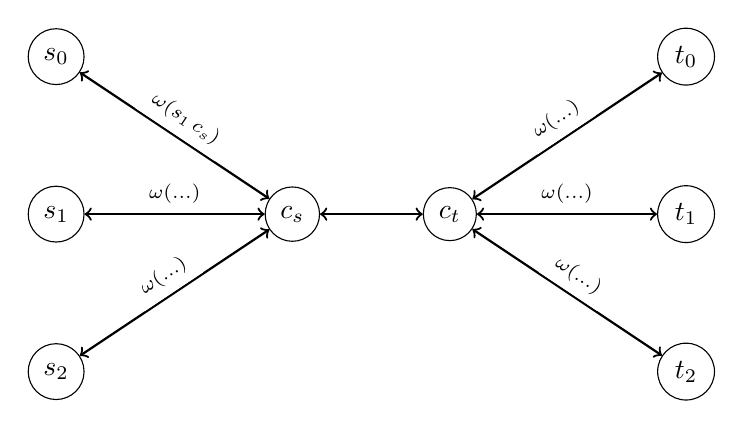
\begin{tikzpicture}

\tikzset{EdgeStyle/.style={<->,font=\scriptsize,above,sloped,midway}}
  \SetGraphUnit{5}
  
  \node[draw,circle] (s3) at (0, 0) {$s_2$}; 
  \node[draw,circle] (s2) at (0, 2) {$s_1$}; 
  \node[draw,circle] (s1) at (0, 4) {$s_0$}; 

  \node[draw,circle] (t3) at (8, 0) {$t_2$}; 
  \node[draw,circle] (t2) at (8, 2) {$t_1$}; 
  \node[draw,circle] (t1) at (8, 4) {$t_0$}; 
  

  \node[draw,circle] (cs) at (3, 2) {$c_s$}; 
  \node[draw,circle] (ct) at (5, 2) {$c_t$}; 

  
  \Edge[label = $\omega(s_1\,c_s)$](s1)(cs)
  \Edge[label = $\omega(...)$](s2)(cs)
  \Edge[label = $\omega(...)$](s3)(cs)
  
  \Edge[label = $\omega(...)$](ct)(t1)
  \Edge[label = $\omega(...)$](ct)(t2)
  \Edge[label = $\omega(...)$](ct)(t3)
  
  \Edge(cs)(ct)

  
\end{tikzpicture}
}

  \end{center}
	
      Since the central arc appears in every route, its value do not matter when considering the process time of an assignment.
      Moreover an assignment without collisions is also an assignment without collisions if the weight of the central arc 
      is set to $0$, therefore we assume from now on it is indeed $0$.
      
      
      Collisions between messages can only appear in the arc $(c_s,c_t)$ on the way forward and in the arc $(c_t,c_s)$
      on the way back. The flow of messages in a star topology is completely described by their repartition in two 
      time window of size $P$ that we call the {\bf forward period} (at $(c_s,c_t)$), and the {\bf backward period} (at $(c_t,c_s)$).
      
%       
%       on the way forward and after node $c_t$ on the way back.
%       Thus, we only have to check if there is no collisions in a given period at those two vertices.
%       We try to order the messages such that they can pass thought the common arcs in a time window of $P$ max. We define the {\bf forward period}, a time window of size P at the beginning of the arc after $c_s$, and the {\bf backward period} the one at the beginning of the arc after $c_t$. A message issued on the route $r$ at time $m_s$ will reach $c_s$ at time $m_{s} + t(c_s,r) \mod P$ in the forward period. If the offset of $\rho(s)$ is $m_{\rho(s)}$, the answer will reach $c_t$ at time $m_{\rho(s)} + t(c_t,\rho(r))\mod P$ in the backward period.
% 
%       A $(P,\tau)$-periodic assignment is then a choice for all $i < n$, of $m_{r_i}$ and $m_{\rho(r_i)}$ such that, for any couple $(i\neq j)$, we have $[t(c_s,r_{i})] \cap [t(c_s,r_{j})] = \emptyset$ and $[t(c_t,\rho(r_i))] \cap [t(c_t,\rho(r_j))] = \emptyset$.

      

  \subsection{Solving PAZL}
  
  In this subsection, we deal with a simpler version of the problem PALL.
  We ask for a $(P,\tau)$-periodic assignment {\bf with all waiting times equal to $0$} and we call this restricted problem {\bf Periodic Assignment for Zero Latency} or PAZL. We consider PAZL since it is simpler to get theoretical results and good algorithms 
  than for PALL. Moreover, as we show in our experimentations of Sec.\ref{sec:exp_PAZL}, this problem can often be solved positively (albeit less often than the general problem). Finally, a solution to PAZL is simpler to implement in real telecommunication networks, since we do not need to implement any buffering at all.    
  
  When the waiting times are zero, $MT({\cal M})$ is equal to twice the weight of the longest route, thus $T_{max}$ is not relevant anymore. For a route $r$, choosing the offset $m_r$ also sets the offset of the route $\rho(r)$ $m_{\rho(r)} + \lambda(r) \mod P$.
  Consider an assignment $\{m_0,\dots,m_{n-1}\}$ of a star topology and let $m_i'= m_{i} - t(c_s,r_i) \mod P$.
  Then $\{m_0',\dots,m_{n-1}'\}$ is an assignment of the same star topology where the weights of the arcs from $s_i$ to $c_s$ are $0$
  for all $i$. Therefore we assume from now on that the \emph{weight of the arcs from $s_i$ to $c_s$ are all equal to $0$}.
  
  
  One may consider a variant of PAZL where the central link is unidirectional, that is collisions can happen between messages going from $c_s$ to $c_t$ and messages  going from $c_t$ to $c_s$. This problem can be shown to be $\NP$-complete by a reduction from the subset sum problem as it is done for a similar problem of scheduling pair of tasks~\cite{orman1997complexity}. We conjecture that the problem PAZL is also $\NP$-complete,  but we have yet not been able to prove it.
  On the other hand we show positive results:  when the period is large or when the routes are short there is always a solution to PAZL and it can be found in polynomial time. We then give an exponential time exhaustive search algorithm which always finds a solution if there is one. 
  
    \subsubsection*{Shortest-longest policy}
    

    We first present a simple policy, which works when the period is large with regard to the weight of the routes.
    The messages are sent in order from the shortest route to the longest route, without any gap between two messages in the forward period.
    In other words, we assume that the route $r_i$ are sorted by increasing $\lambda(r_i)$ and we set $m_{i}$ the offset of $r_i$ to $i\tau$. We call this algorithm {\bf Shortest-Longest}.
      
     By definition, there are no collision in the forward period and if the period is long enough, 
     it is easy to see that in the backward period the order of the messages are the same as in the forward period and that no collision can occur. 
      
      
      \begin{proposition} Let $(G, {\cal R})$ be a symmetric routed network, and let $n\tau + 2(\lambda(r_{n}) - \lambda(r_{0})) \leq P$, then there is $(P,\tau)$-periodic assignment of $(G, {\cal R})$ with all waiting times $0$ which is given by Shortest-Longest in time $O(n\log(n))$.\label{prop:SL}
      \end{proposition}
      \begin{proof}
       Since $m_{s_i} = i\tau$, $[t(c_s,r_{i})] = \{i\tau,\dots, (i+1)\tau -1\}$ and there are no collision on the forward period.
       
       
       We may assume that $\lambda(r_{0}) = 0$, since removing $\lambda(r_{0})$ from every arc $(c_t,t_i)$ does not change the order on the length of the routes nor the collisions between messages.
       Since $\lambda(r_{0}) = 0$, by hypothesis we have $n\tau + 2\lambda(r_{n}) \leq P$ which implies that
       $[t(c_t,r_{i})] = \{2 \lambda(r_{i}) + i\tau, \dots,  2 \lambda(r_{i}) + (i+1)\tau -1\}$.
       Since $ \lambda(r_{i}) \leq  \lambda(r_{i+1})$ by construction, we have  $2 \lambda(r_{i}) + i\tau -1 < 2 \lambda(r_{i+1}) + (i+1)\tau$ which proves that there are no collision on the backward period. 
       
       The complexity of the algorithm is dominated by the sorting of the routes in $O(n\log(n))$. 
      \end{proof}

      If the period is slightly smaller that the bound of Proposition~\ref{prop:SL}, a collision will occur on the first route in the backward period. Hence, this policy is not useful even as a heuristic for longer routes as confirmed by the experimental results of Subsection~\ref{sec:exp_PAZL}. 

   
    \subsubsection*{Greedy algorithm}
    
    We propose a greedy algorithm to build a $(P,\tau)$-periodic assignment, which provably works when
    the period is large enough with regard to the number of routes and size of messages. In other words, 
    we can always find a solution when the network is far from saturated. This algorithm defines an upper bound for the period. As a reminder, the lower bound is $n\tau$, that is, the size taken by the messages to be emitted.
    
    \begin{proposition}
     Let $(G, {\cal R})$ be a symmetric routed network, and let $ 3n\tau \leq P$, then there is $(P,\tau)$-periodic assignment of $(G, {\cal R})$ with all waiting times $0$ which can be found in time $O(n^2)$.
    \end{proposition}
    \begin{proof}
     We consider the forward period and cut it into consecutive interval of size $\tau$ that we call macro-slots. The algorithm works by choosing an offset for each route in the following way: try all offsets which put the message in a yet not used macro-slot in the forward
     period. The choice of an offset also fixes the position of the message in the backward period, chose the first one which does not create a collision. We now prove that this algorithm always finds a $(P,\tau)$-periodic assignment without waiting time when $P \geq 3n\tau$.
     
     Assume we are choosing the offset of the route $r_{k+1}$, we have at least $P - k \geq 3n - k$ free macro-slots in the forward period, since $P \geq 3n\tau$. Each of these $3n - k$ possible offset values translates into $3n - k$ positions of messages in the backward period. All these positions are separated by at least $\tau$ slots. There are already $k$ messages of size $\tau$ in the backward period. One such message can intersect at most $2$ potential positions since they are disjoint intervals. Therefore  amongst the possible $3n - k$ positions, there are  at least $3n - k -2k$ which are without collision. Since $k < n$, $3n - k -2k \geq 1$, which proves that the algorithm terminates and find a  $(P,\tau)$-periodic assignment. 
     
     This algorithm works with a complexity $O(n^2)$, since for the $k^{\text{th}}$ route we have to try at most $2k$ offsets before finding a correct one. We can test the $2k$ offsets of the backward period in time $O(k)$ by maintaining an ordered list of the intervals used by already set routes.
     \end{proof}
     
      \begin{center}
      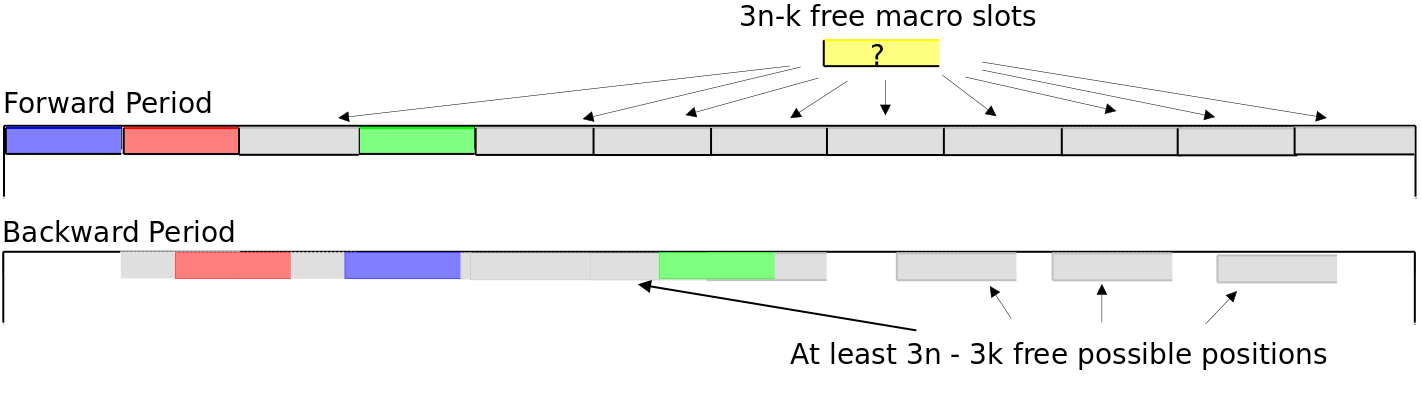
\includegraphics[width=\textwidth]{ex3nt.png}
      \end{center}
% 	\begin{algorithm}[H]
% 	\caption{Greedy assignment}
% 	\begin{algorithmic}
% 	\REQUIRE ${\cal R}_{\cal C}$, period $P$
% 	\ENSURE A P-periodic assignment in p $\leq P$, or FAILURE
% 	\STATE $T$ a table of the macro slots of size $\tau$ in the forward period.
% 	\STATE $L$ a list of free intervals in the backward period%$P2[P]$ slots backward period.
% 	\FORALL{source $s$ in S}
% 
% 	\FORALL{free intervals $[a,b]$ in $L$}
% 	\FORALL{ $a/\tau - \lambda(s) <j< b/\tau - \lambda(s)$ }
% 	\IF{ $T[j] == FREE$}
% 	\STATE $m_{s} \leftarrow j.\tau$
% 	\STATE $T[j] = USED$
% 	\STATE update $[a,b]$ in $L$
% 	\STATE BREAK
% 	\ENDIF
% 	\ENDFOR
% 	\ENDFOR
% % 	
% % 	\IF{No intervals are found for $s_i$}
% % 	\STATE return FAILURE
% % 	\ENDIF
% % 	\ENDFOR
% 
% 	\ENDFOR
% 
% 	\end{algorithmic}
% 	\end{algorithm}
	
This algorithm, contrarily to the previous one, may work well, even when the condition $P \geq 3n\tau$ is not true.
In fact, experimental data in Subsection~\ref{sec:exp_PAZL} suggests that the algorithm finds a solution on average when $P \geq 2 n\tau$.
Note that we also experimented with other greedy algorithms which do not use macro-slots, they work even better in practice but their theoretical upper bound is worse.

	\subsubsection*{Exhaustive search}
% 	\begin{algorithm}[H]
% 	\caption{Exhaustive Generation}  
% 	\begin{algorithmic}
% 	\REQUIRE A routage graph ${\cal R}_{\cal C}$, period $P$, packet size $\tau$
% 	\ENSURE $(P,\tau)$-periodic assignment of ${\cal R}_{\cal C}$
% 	\STATE Forward-budget $\leftarrow$ $P$ - n * $\tau$
% 	\STATE Backward-budget $\leftarrow$ $P$ - n * $\tau$
% 	\STATE Free-Intervals $\leftarrow$ list of free intervals in the backward period, init to $[0;P[$
% 	\FORALL{source $s_i$ in S}
% 	\FORALL{j in Free-Intervals }
% 	\IF{Message of the route $r_{s_i}$ does not collides with scheduled routes}
% 	\STATE $m_{s_i} \leftarrow $ the first slot of Free-Intervals[j]
% 	\STATE Split the Free-Intervals considering the new packet
% 	\STATE Forward-budget $\leftarrow$ Forward-budget - {\em lost size}
% 	\STATE Backward-budget $\leftarrow$ Backward-budget - {\em lost size}
% 	\STATE call Exhaustive Generation on remaining routes
% 	\ENDIF
% 	\ENDFOR
% 	\ENDFOR
% 
% 
%       \end{algorithmic}
%       \end{algorithm}

% 	    
      We now present an exhaustive search algorithm, which tries to set the offsets in all possible ways until it has found a $(P,\tau)$-periodic assignment. Contrarily to the two previous algorithms, when it fails to find a solution, then it certifies there are no solution to PAZL.
      
      We have $n$ routes denoted by $\{0,\dots,n-1\}$. A partial solution $S$ is 
      a partial function from $[n]$ to $\{0,1,\dots,P-\tau -1\}$ which sets a starting time for a subset of the routes $R(S) \subseteq [n]$, such that there are no collisions for these routes.  A partial solution $S'$ extends $S$, if $S'$ is defined over one more route than $S$ and this route has a larger starting offset than all routes of $S$: $R(S') = R(S) \cup \{r'\}$ and for all  $r \in R(S)$, $S(r) + \tau \leq S'(r')$. We define a tree whose nodes are partial solutions and such that the root is the empty partial solution and the children of a partial solution are the partial solutions which extend it. The solutions to our problem will be the leaves of depth $n$ in the tree, and our exhaustive search algorithm is a depth-first search of this tree. 
      
      Remark that a node $S$ with $|R(S)| = k$ can have as many as $(n-k)P$ children. Since the tree is of depth $n$, the tree may have as many as $n!P^n$ elements and while $n$ is small, $P$ may be large which makes its traversal intractable.  Therefore we have to find cuts in the tree to avoid to explore it entirely and henceforth make the algorithm practical. Cuts correspond to the detection of subtrees which contain no solutions or solutions which can be found elsewhere and can thus be skipped. We now propose three cuts, the first two being particularly useful when the network is loaded ($n\tau$ is not far from $P$). 
      
      \begin{enumerate}
       \item We consider the number of slots which can be used by routes not yet fixed by a partial solution in the \emph{forward period}. When we extend a solution into $S$ with a new route at offset $m$, then at most $(P - m) / \tau $ routes can still be used to extend $S$ without collisions in the forward period. If that value is less than the number of routes which are not in $R(S)$, it is a failure and the algorithm backtracks.
       
       \item 
       For the next two cuts, we need to define the notion of the useful slots of a partial solution $S$ in the \emph{backward period}: a slot is said to be useful, if it is not used by a message set by $S$ in the backward period and it belongs to an interval of at least $\tau$ such slots. Useful slots are positions of the backward period which can be used when extending $S$. We will denote by $([a_i,b_i[)_{i\leq l}$ the ordered sequence of intervals of useful slots of $S$. Without loss of generality we can assume that all $a_i, b_i \leq l$. The number of messages of size $\tau$ which can be placed in the useful slots of $S$ is thus  $\displaystyle{ \sum_{i=0}^{l} (b_{i} -a_i)/\tau } $. If that value is less than the number of routes which are not in $R(S)$, it is a failure and the algorithm backtracks. Notice that the list of intervals of useful slots and the value $\displaystyle{ \sum_{i=0}^{l} (b_{i} -a_i)/\tau } $ can be maintained in constant time, since each time a route is added, we only need to split an interval of useful slots into at most two such intervals.
       
       \item 
       Let $S_1$ and $S_2$ be two partial solutions with $R(S_1) = R(S_2)$. Let $US_1$ (respectively $US_2$) be the set of useful slots of $S_1$ (resp. $S_2$). We say that \emph{$S_1$ dominates $S_2$} if there are more useful slots both in the forward and backward periods for $S_1$ than for $S_2$. Formally, the largest offset fixed in $S_1$ is smaller than the one in $S_2$ and $US_2 \subseteq US_1$. Remark that any valid sequence of extensions of $S_2$ (choosing offsets of routes in the complementary of $R(S_2)$) is also a valid sequence of extensions of $S_1$. Therefore if the tree rooted at $S_2$ contain a solution, then $S_1$ contains one too. Hence, in our exhaustive search of the tree of partial solutions, we can skip the tree rooted at $S_2$.
       
       We now explain how we can detect some partial solutions which are dominated so that we do not explore their subtrees.
       Consider a partial solution $S$ which we extend into $S'$ by setting the offset of the route $r$ to be the smallest possible. The offset of $r$ in the backward period is $S'(r)+ \lambda$ and we denote the end of the message before before by $a$. Hence all extensions of $S$ into $S''$ such that $S'(r)  < S''(r) < a + \tau - \lambda$ are dominated by $S'$. Therefore when computing the extension of $S$, we first build $S'$ and then $S''$ with $S''(r) =  a + \tau - \lambda$ , skipping all values in between.
       
       \end{enumerate}
      
      The third cut works well in conjunction with the first one since it makes the offsets grow quickly and 
      which makes the first cut more likely to apply. A last cut could be implemented: compute for every route not in $R(S)$ the set of possible positions in the backward period and verify whether at least one is contained in the useful slots of $S$.


    \subsection{Experimental evaluation}\label{sec:exp_PAZL}
      
      The following experimental results compare the three presented algorithms.
      Notice that both Greedy algorithm and Shortest-Longest are polynomial time algorithm but are not always able to find a solution, depending on $P$, $\tau$, $n$ and the size of the routes. On the other hand, the exhaustive search will find an optimal solution if it exists, but works in exponential time. We will compare the performance of the algorithms in two different regimes: routes are either short with regard to $\tau$, or unrestricted.
      From our C-RAN context we choose the following parameters: the number of routes 
      is at most $n = 20$, $\tau$ is equal to $2500$. Moreover the period is always larger than $n\tau$ otherwise no assignment is possible and smaller than $3n\tau$ otherwise the greedy algorithm always returns a solution. 
      The code in C is available online on the webpage of one of the authors~\cite{webpage}.
      
      We can define the load of the network as $\frac{n\tau}{P}$ (here a value between one and three) and in experiments we will try to understand how our algorithms work with regards to the load. Often rather than changing the load, we will change the period which is equivalent. 
      

      \paragraph{Short routes}
      
      First we consider routes which are shorter than $\tau$, that is a message cannot be contained 
      completely in a single edge which is very common for our application. We generate star topologies in which the weights of the arcs $(c_t,t_i)$ are drawn uniformly between $0$ and $700$ slots. It corresponds to messages of approximately $1$ Mb, links of bandwidth $10$ Gbps and length less than $5$ km between the BBU and the RRH. 
      
      Our aim is to understand how well the algorithms are working under high load. To do that we try to evaluate the 
      minimal period (that is the highest possible load) for which a $(P,\tau)$ periodic assignment can be found by each algorithm. 
      To that end we use a linear search on $P$, since a dichotomy method would not work because of Lemma~\ref{lemma:monotonic}.
      
      In our experiment, we generate $1000$ random instances of PAZL for $1$ to $12$ routes. 
      We measure the average minimal period, for each algorithm. The experiments are stopped at $12$ routes because the exhaustive search algorithm becomes too slow for larger $n$. Remind that the exhaustive search always finds the best possible period for a given instance. The lower and upper bound $n\tau$ and $3n\tau$ are also represented.
      
      
        
      \begin{figure}

      \begin{center}
	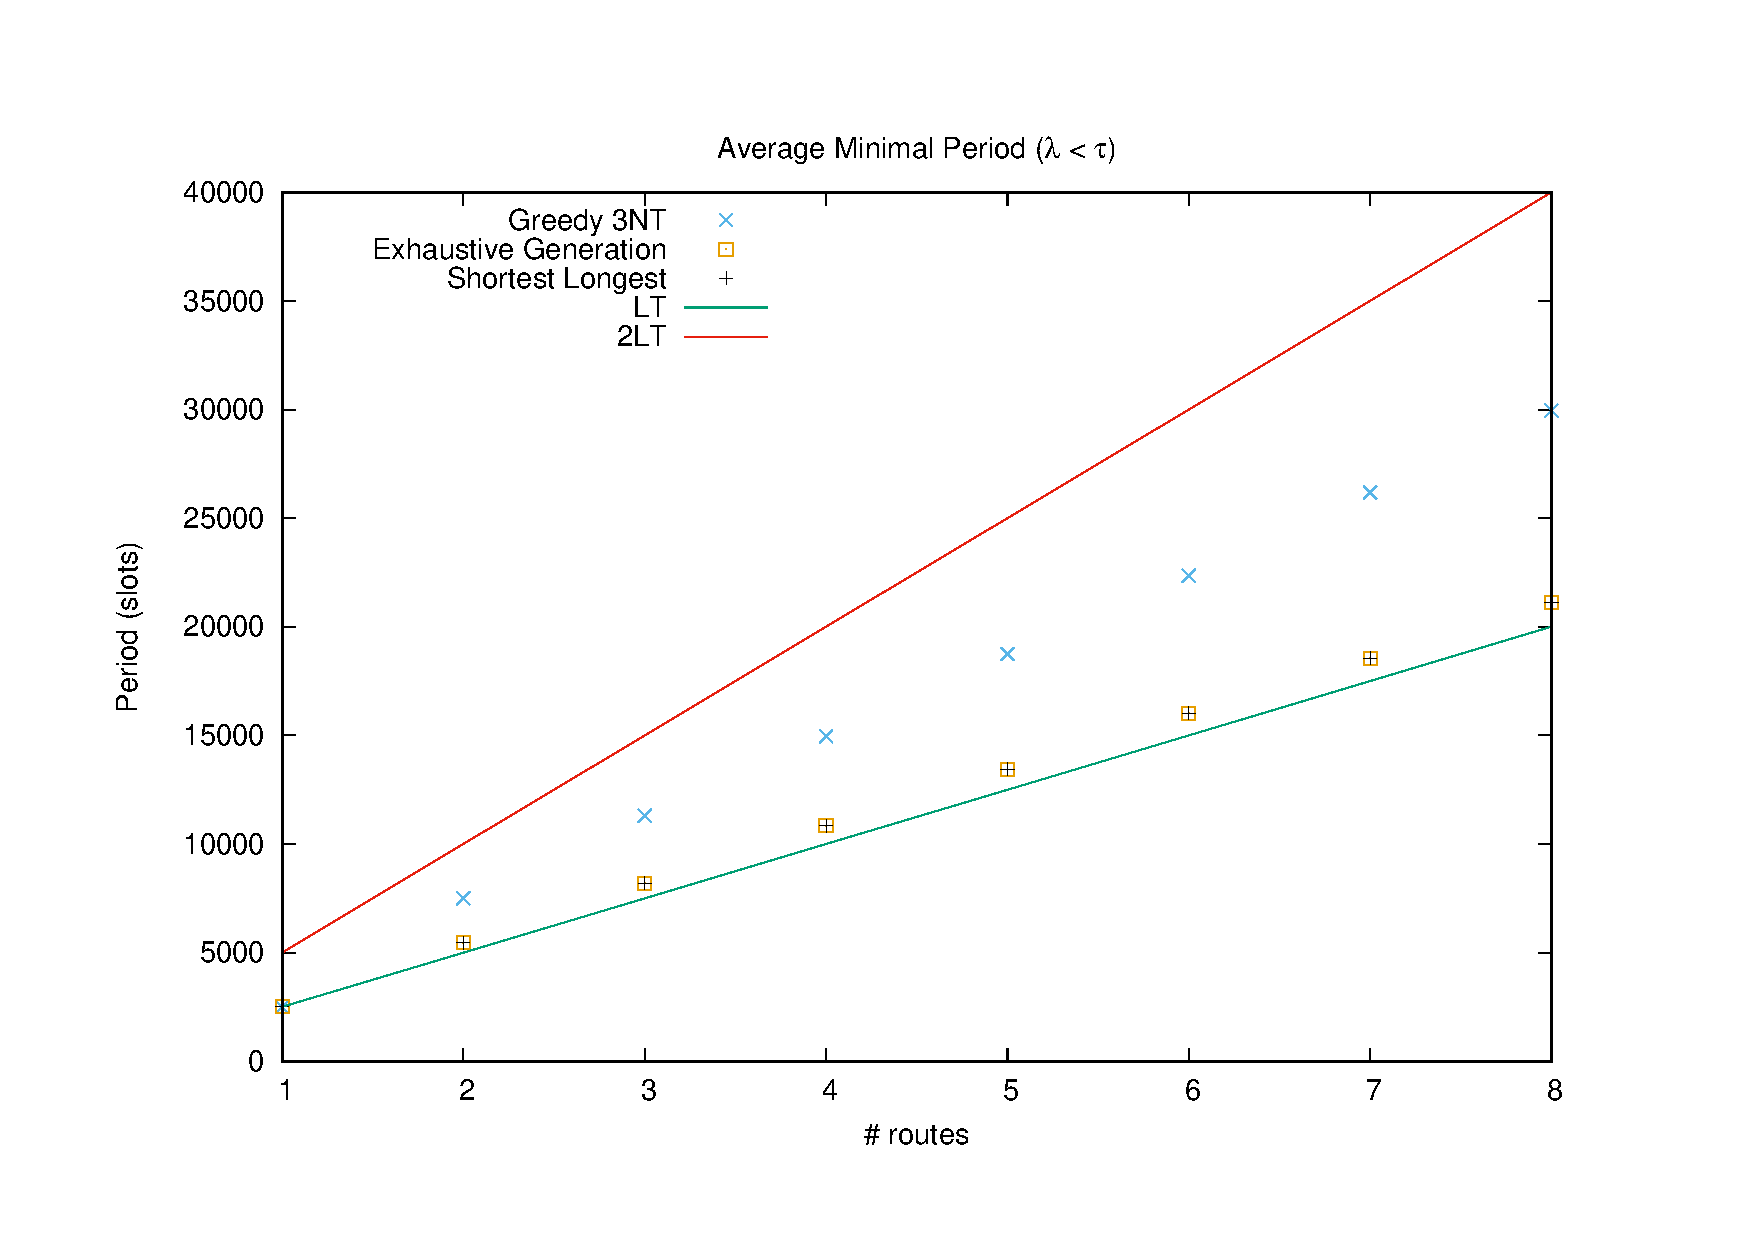
\includegraphics[scale=0.4]{periode_petite.pdf}
      \end{center}
      \caption{Minimum period averaged over $1000$ random instances}
      \end{figure}
      
      First, we remark that the period found by the exhaustive search is only very slightly above the lower bound of 
      $n\tau$, which means that, in this regime, it is very well justified to look for a solution without waiting time even for a highly loaded network. 
      
      The period needed by the Shortest-Longest algorithm to find an optimal solution is a function of the difference between the longest and the shortest route and its average could be easily determined theoretically. The algorithm was expected to find a period close to the optimal one since the routes are short. It turns out it always finds the optimal period in our experiments. Therefore, we should use it in practical applications with short routes, instead of the exhaustive search which is much more computationally expensive. 
      
      Finally we remark that the greedy algorithm has an average period much lower than the theoretical upper bound of $3n\tau$. We made a linear regression on this value and with a correlation coefficient greater than $0,999$ we find a slope of $1.53n\tau$.
      
      

      \paragraph{Long routes}
      
      We now want to understand the performance of these algorithms when the size of the routes is unbounded. When the routes are long, the cuts in the exhaustive search are less efficient and thus even for a small number of routes the algorithm may be impractical. To make the experimentations short enough, we have bounded the number of nodes of the tree of partial solutions the exhaustive search can visit by $10^9$.
      
      In this experiment we will fix the number of routes to $8$ and the weights of the arcs $(c_t,t_i)$ are drawn following an uniform distribution between $0$ and $30000$ slots (in the same range as the period).
      We measure for each algorithm its percentage of success, for periods from $20000$ which is the minimum possible to $50000$.
      
      The exhaustive search can fail because there are no solutions or because it does not have enough time to finish its calculation. Hence we represent both the success rate of the algorithm, and an upper bound on the success rate of any algorithm solving PAZL by combining the successes and the failures because of lack of time of the exhaustive search. 
      
\begin{figure}

       \begin{center}
      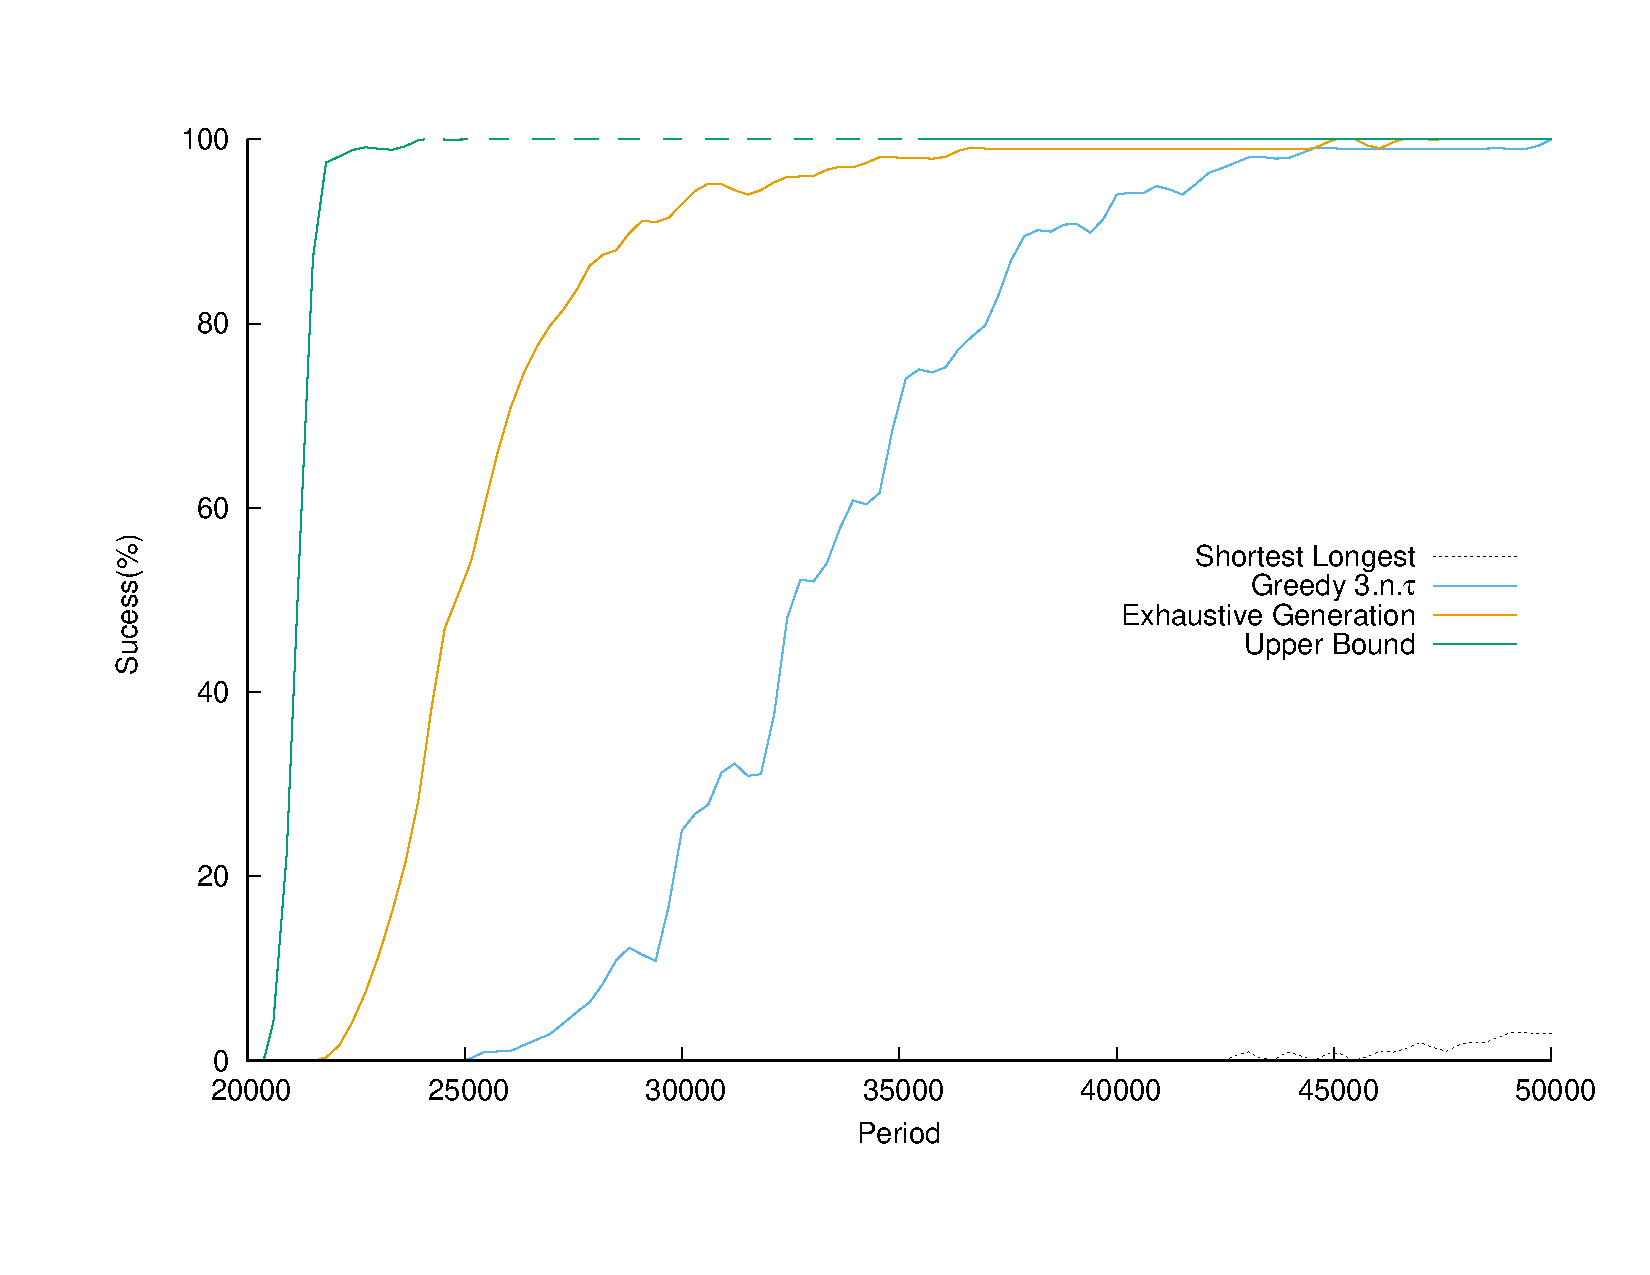
\includegraphics[scale=0.4]{echec_longues.pdf}
      \end{center}
      \caption{Success rate for $8$ routes over $1000$ random instances}
     \end{figure}
      
      In this regime, the performances of Shortest-Longest are abysmal since it depends on the difference between the longest and the smallest route which is large here. On the other hand, the greedy algorithm has a performance not so far from the case of short routes, which is expected since it does not directly depend on the size of the route. When repeating the experiments of the previous section on routes of arbitrary length, we find that on average the greedy algorithm finds a solution if $P>1.89n\tau$.
      
      When the period is less than $40000$, the exhaustive search find many more solutions than the greedy algorithms which justifies its use. However for small period, less than $30000$ the computation time is really important and without improvements it would not be possible to tackle larger problems with $10$ to $20$ routes. Moreover, examining the upper bound curve for periods less than $22000$, we see that there are very few instances with a solution for PAZL. It means that with long routes and high load (larger than $0.9$), looking for an assignment without waiting time is far too restrictive. That is why we present algorithms for the general PALL problem in our next section. We will test them on $8$ long routes and a period between $20000$ and $30000$ where, as we have shown here, there are often no easy to compute assignment without waiting times.
      
   \section{The Star Topology: Minimizing Latency}\label{sec:PALL}
    
    In this section, we still work on the star topology, but we consider again the more general PALL problem. It means that the messages can wait in the target vertices (BBUs) in order to find solutions when there are none without waiting time. We allow the process times $PT$ of the routes to be greater than twice the weights of the routes, but it should less than $T_{max}$.

	\subsection{Special cases}
		
		
	Often in real networks, the length of the routes are not arbitrary and we may exploit that to solve PALL easily. For instance if all the weights on the arcs $(c_t,t_i)$ are the same, we can replace them all by $0$ and substract this weight to $T_{max}$.
	The assignment in that case is trivial, just send all messages so that they follow each other without gaps in the central arc $(c_s,c_t)$. Since the arcs $(c_t,t_i)$ are of weigth $0$, all messages will go through $(c_t,c_s)$ on their way back in
	the same order and thus will not collide. 
	
	
	A more realistic assumption would be that all weigths of the arcs $(s_i,c_s)$ are the same. It would correspond to a situation where all the BBUs are in the same datacenter.
	
	 \begin{theorem}
	 Let $(G,{\cal R})$ be a symmetric routed network with $n$ routes and let $P \geq n\tau$. If there is a constant $c$ such that $\forall i < n, \,\omega(s_i,c_s) = c$, then there is a $(P,\tau)$-peridoic assignment with process time $2 \times \displaystyle{\max_{r\in {\cal R}} \lambda(r)}$ and it can be built in time $O(n)$.
	 \end{theorem}
      \begin{proof}
      
        We can simplify the weights on the arcs $(s_i,c_s)$ by setting them all to $0$.
        We find the route with maximal length, say that it is $\lambda(r_0)$. The idea is to 
        set the waiting times of all routes so they behave exactly as the message in $r_0$.
        
        The offset of the route $r_i$ is set to $i\tau$, which ensures that there are no collision on the way forward (on the arc $(c_s,c_t)$) as soon as $P \geq n\tau$ which is the minimal possible period. We set the waiting time for the route $i$ to $w_i = 2(\lambda(r_{0}) - \lambda(r_{i}))$. We can compute the time at which the message of the route $r_i$ arrives at the vertex $c_t$ on its way back: $t(r_i,(c_t,c_s)) = w_i + i\tau + 2\lambda(r_{i})$
        by replacing $w_i$ by its value we obtain $t(r_i,(c_t,c_s)) =  i\tau + 2\lambda(r_{0})$
        As a conclusion there are no collision on the edge $(c_t,c_s)$ as soon as the 
        period is larger than $n\tau$ (there are no gaps between the messages).
        
        Now let us compute the process time of the route $r_i$ defined by $PT(r_i) = w_i + 2\lambda(r_{i}) $. We obtain $PT(r_i) = 2\lambda(r_{0})$ and thus the maximum process time of the assignment is also equal to $2\lambda(r_0)$.
	Finally the complexity is $O(n)$ since we have to find a maximum between the size of $n$ routes and the computation of each $w_i$ is done by a constant number of artihmetic operations.
     \end{proof}
     
     Remark that this assignment always exists and has no collision when $P \geq n\tau$. 
     If for any pair of indices $(i,j)$ the difference between the weights of the arcs $(s_i,c_s)$ and $(s_j,c_s)$ is bounded 
     by $d$ and the length of the longest route is $l$, then the maximum process time is bounded by  $2l + d$.

     
     \subsection{A two stage approach}
     
     We can decompose any algorithm solving the PALL problem in two parts: first set the offsets of the forward routes and then knowing this information set the offset of the backward routes or equivalently the waiting times.  
     The offsets of the forward routes will be chosen so that all messages have no collision on the central arc and such that there are no free slots inbeetween the end of a message on the central arc and the beginning of the next one. 
     It is done to minimize the period needed to send the messages of the forward route.
     We tried the five following orders. 
	\begin{itemize}
	 
	 \item Longest-Shortest on Routes (LSR): Decreasing order on the length of the routes.
	 \item Shortest-Longest on Routes (SLR): Increasing order on the length of the routes. 
	 \item Longest-Shortest on last Arc (LSA): Decreasing order on the length of the arcs $(c_t,t_i)$.
	 \item Shortest-Longest on last Arc (SLA): Increasing order on the length of the arcs $(c_t,t_i)$. This sending order yields a $(P,\tau)$ periodic assignment in which all the $w_i = 0$, if the period is large enough (see proposition \ref{prop:SL}).
	 \item Random: A random order of the routes.
	\end{itemize}

   In the rest of the section we will study different methods to compute the offsets of the backward routes, once
   the offsets of the forward routes are fixed by one of the previous orders.
   
   \subsection{Greedy scheduling of backward routes}
    
    Assume that the offsets of the forward routes are fixed by some order. 
    Consider a forward route $r_i$ and the corresponding backward route $r_{\rho(i)}$.
    We define the {\bf deadline} of $r_{\rho(i)}$ as $m_{i} + T_{max} - \omega(s_i,c_s)$, that is the latest time at which the message can go out of $c_t$ such that $PT(r_i) \leq T_{max}$.
    We say that a backward route $r_{\rho(i)}$ is {\bf eligible} at time $t$ if $m_{i} +  \lambda(r_i) + \omega(c_t,t_i) \leq t$, that is the message of the route $r_{\rho(i)}$ arrives at $c_t$ before time $t$ when $w_i = 0$.
    
    The first algorithm we propose is a greedy algorithm which sets the offset of the 
    backward routes. It prioritizes the routes with the earliest deadline to best satisfy the
    constraint on the process time.
    Set $t=0$ and repeat the following: find $s \geq t$ the first time for which there is an eligible route with its offset not fixed. Then amongst all eligible routes at time $s$ choose the one with the smallest deadline, fix its offset to $s$ and set $t = s + \tau$.
    
    This algorithm does not take into account the periodicity. Say that $t_0$ is the smallest offset that the algorithm has fixed
    for a backward route. Then for all routes with an offset smaller than $t_0 + P - \tau$,
    by construction, there are no collisions on the central arc.
    However, for routes with larger offsets, since we  should consider everything modulo $P$, 
    they may collide with any other route. Therefore we must adapt the greedy algorithm of the previous paragraph by finding $s \geq t$ the first time for which there is an eligible route with its offset not fixed and \emph{such that there is no collision if a message go
    through the central arc at time $s$}. 
    
     \begin{algorithm}[H]
    \caption{ Greedy deadline ({\bf GD}) }
    \begin{algorithmic}
    \REQUIRE A routed network $(G,{\cal R})$, a period $P$, packet size $\tau$, $ T_{max}$, the offsets $m_i$
    \ENSURE $(P,\tau)$-periodic assignment of $(G,{\cal R})$, or failure
   \STATE  ${\cal H} \leftarrow$ empty set //{\em set of eligible routes}
       \STATE  free\_ intervals $\leftarrow$ [0,$P$] //{\em list of intervals of free slots}
  
    \FORALL{route $r_{i}$}
    \STATE  deadline[$r_i$]  $\leftarrow$  $m_{i} + T_{max} - \omega(s_i,c_s)$
    \STATE  eligible\_time[$r_i$] $\leftarrow$ $m_{i} +  \lambda(r_i) + \omega(c_t,t_i)$
      \ENDFOR
      
      \WHILE{There is some non-assigned routes}
      \IF{${\cal H}$ is empty}
      \STATE t $\leftarrow $ min\_non\_assigned(eligible\_time)
      \STATE take $r_i$ the route with eligible\_time[$r_i$] = t
      \STATE 
      \ENDIF
      
      \STATE $r \leftarrow $ extract\_min(${\cal H}$)
      \STATE t $\leftarrow$ next\_free\_interval(free\_intervals, t) //{\em if there is no more free intervals of size $\tau$, the algorithm fails}
      \STATE $w_i \leftarrow$ t - eligible\_time[$r_i$]
      \STATE update(t,free\_ intervals)
      \STATE t $\leftarrow$ t + $\tau$
      \FORALL{routes $r_i$ with  eligible\_time[$r_i$] $\leq$ t}
      \STATE insert ( ${\cal H}$,$r_i$).
      \ENDFOR
      \ENDWHILE
%    \STATE  $w_i \leftarrow 0$
%    \FORALL{route $r_{t_i}$}
%    \STATE  $w_i \leftarrow 0$
%    \STATE period-end $\leftarrow m_{s_i} + \lambda(r_{s_i}) + t(c_t,r_{t_i}) + P$
%    \FORALL{route $r_{t_j}$}
%    \STATE deadline-route$ \leftarrow m_{s_j} + T_{max}-t(c_s,r_{s_j})$
%    \STATE $deadline \leftarrow$ min(deadline-route,period-end)
%    \ENDFOR
    

    \end{algorithmic}
    \end{algorithm}
    The function  min\_non\_assigned(eligible\_time) returns the lowest time in eligible\_time, for which the corresponding route is not assigned yet. The function update(free\_intervals) removes an interval of size $\tau$ beginning at t, which correspond to the message,  from free\_intervals.


    The greedy algorithm can be made to work in time $O(n\log(n))$. 
    To do that the set of eligible routes must be maintained in a binary heap
    to be able to find the one with smallest deadline in time $O(\log(n))$. 
    To deal with the possible collisions, one can maintain a list of the intervals
    of time at which a message can be send on the arc $(c_t,c_s)$. Each time the offset of a 
    route is fixed an interval is split into at most two intervals in constant time. 
    Since the algorithm goes over the elements of the list at most twice when doing an insertion
    or looking for the next free interval, the time needed to maintain it is $O(n)$. 
    
%     
%          We compared the two algorithms on $10000$ graphs on which the weight of the links are drawn uniformly between $0$ and $20000$, with a period of $21000$, and giving, for each instance $T_{max} = 2\lambda(r_{longest-route})$ . We then look at the success rate of each algorithms, with every sending order. Both algorithms reach the higher success rate with the Random sending order, but the success of Greedy is $5,65 \%$, while the success rate of Greedy Periodic is to $30,02 \%$.
    

    
     
     \subsection{Earliest deadline scheduling}
     
     
     The problem to solve in the second stage of our approach is very similar to the following scheduling problem: 
     we are given a set of jobs and each job has a \emph{release time} and a \emph{deadline}. 
     The problem is to schedule all jobs on a single processor, that is choosing the time at which they are computed, so that no two jobs are scheduled at the same time. A job is always scheduled after its release time and it must be finished before its deadline. Let us call $n$ the number of jobs, the problem can be solved in time $O(n^2\log(n))$~\cite{simons1978fast} when all jobs have the same running time and it gives a solution with the earliest possible deadline. On the other hand if the running times are different the problem is $\NP$-complete~\cite{lenstra1977complexity}. 
     The  polynomial time algorithm  which solves this scheduling problem is similar to the Greedy algorithm presented in the previous section. However, when it fails because a job finishes after its deadline, it changes the schedule of the last messages to find a possible schedule for the problematic job. The change in the scheduling is so that the algorithm cannot fail on the same job a second time except if there is no solution, hence the polynomiality of the algorithm.
     
     We reduce our problem of setting the offsets of the backwards routes once the order of the forward routes is fixed to this
     scheduling problem. The backward routes are the jobs, the size of a message is the running time of a job,
     the deadline of a route is the deadline of the corresponding job and the smallest time at which it is eligible is the release time. Let us call {\bf Minimal Latency Scheduling (MLS)} this algorithm.
     Remark that we do not deal with the periodicity. When MLS finds a solution ${\cal M}$ its always satisfies $MT({\cal M}) < T_{max}$. On the other hand, it is a $(P,\tau)$ periodic assignment only if $m_n - m_1 \leq P -\tau$ where $m_n$ is the largest offset and $m_1$ the smallest one. The algorithm we use minimize $m_n - m_1 $, so it may work quite well in practice (as shown in Section~\ref{sec:resultsPALL}).
     
     We now present a variant of the previous algorithm that we call {\bf Periodic Minimal Latency Scheduling (PMLS)}
     which takes into account the periodicity. We fix arbitrarily a backward route so that its message is the first to go through the central arc at time $t$. Then we modify the deadline of each forward route to be the minimum of their previous deadline and $t + P$.  We execute this algorithm for every possible first backward route while no solution is found. Since we run the previous algorithm at most $n$ times, the complexity is in $O(n^3\log(n))$. Remark that it will always find more solution than MLS,
     because if MLS find a solution with first route $r$ and such that $m_n - m_1 \leq P -\tau$, then this solution will be found by PMLS when it selects $r$ as the first route. Moreover when PMLS finds a solution, it is always a $(P,\tau)$ periodic assignment
     since we guarantee that all messages are scheduled in a period of time of size $P$ and it satisfies $MT({\cal M}) < T_{max}$ by construction of the deadlines. The scheduling algorithm we use always finds a solution to the  original problem it solves. However, in our periodic context, we do not allow to choose an offset for a route after $t+P- \tau$ which modulo $P$ may not collide with another route. Therefore PMLS may fail while there is a solution.
     
%     \begin{algorithm}[H]
%     \caption{ Minimized Scheduling Periodic (MSP)}
%     \begin{algorithmic}
%     \REQUIRE A routed network $(G,{\cal R})$,a period $P$, packet size $\tau$, $ T_{max}$, the offsets $m_i$
%     \ENSURE $(P-\tau)-$periodic assignment of $(G,{\cal R})$, if it exists
%   
%     \FORALL{route $r_{t_i}$}
%     \STATE  $w_i \leftarrow 0$
%     \STATE period-end $\leftarrow m_{s_i} + \lambda(r_{s_i}) + t(c_t,r_{t_i}) + P$
%     \FORALL{route $r_{t_j}$}
%     \STATE deadline-route$ \leftarrow m_{s_j} + T_{max}-t(c_s,r_{s_j})$
%     \STATE $deadline \leftarrow$ min(deadline-route,period-end)
%     \ENDFOR
%     
%     \STATE Call (MS)
% 
%     
%     \ENDFOR
% 
%     \STATE return the best $(P,\tau)$-periodic assignment, or FAILURE
% 
%     \end{algorithmic}
%     \end{algorithm}
    
    \subsection{Experimental evaluation}
    \label{sec:resultsPALL}
    
    
    In this section, we first try to understand what is the best choice of order for the first stage of the algorithm.
    We fix the number of routes to $8$ to make comparisons with the results of Section~\ref{sec:exp_PAZL} easier. 
    We draw uniformly the weights of the arcs between $0$ and $20000$ slots.
    For a given routed network, we define the {\em margin} as the difference between $T_{max}$ and twice the longest route. 
    Hence, for a routed network choosing the margin or $T_{max}$ is the same, but since we will consider many networks 
    whith different longest route's size, it will be more meaningful to set the margin rather than $T_{max}$.
    In fact the margin represents the latency imposed by the communication process without taking into account the physical length of the network which cannot be changed. In our experiments the margin range from  $0$ to $3000$ slots.
   We look at two different regimes: we take a period equal to $1,05n\tau$ to represent a very loaded network
   and $1,5n\tau$ for a mildly loaded network. Choosing a larger period is not relevant since then we know how to solve the problem even without waiting times as shown in Section~\ref{sec:exp_PAZL}. We represent the success rate with regards to the margin, for the five kind of orders using the Greedy algorithm for the second stage, computed over $10000$ random star topologies. Note that for the random order, we compute $1000$ random orders and count it as a success as soon as there is a solution for one order. 
 
\begin{figure}[H] 
    \begin{minipage}[c]{6cm}
  \centering
      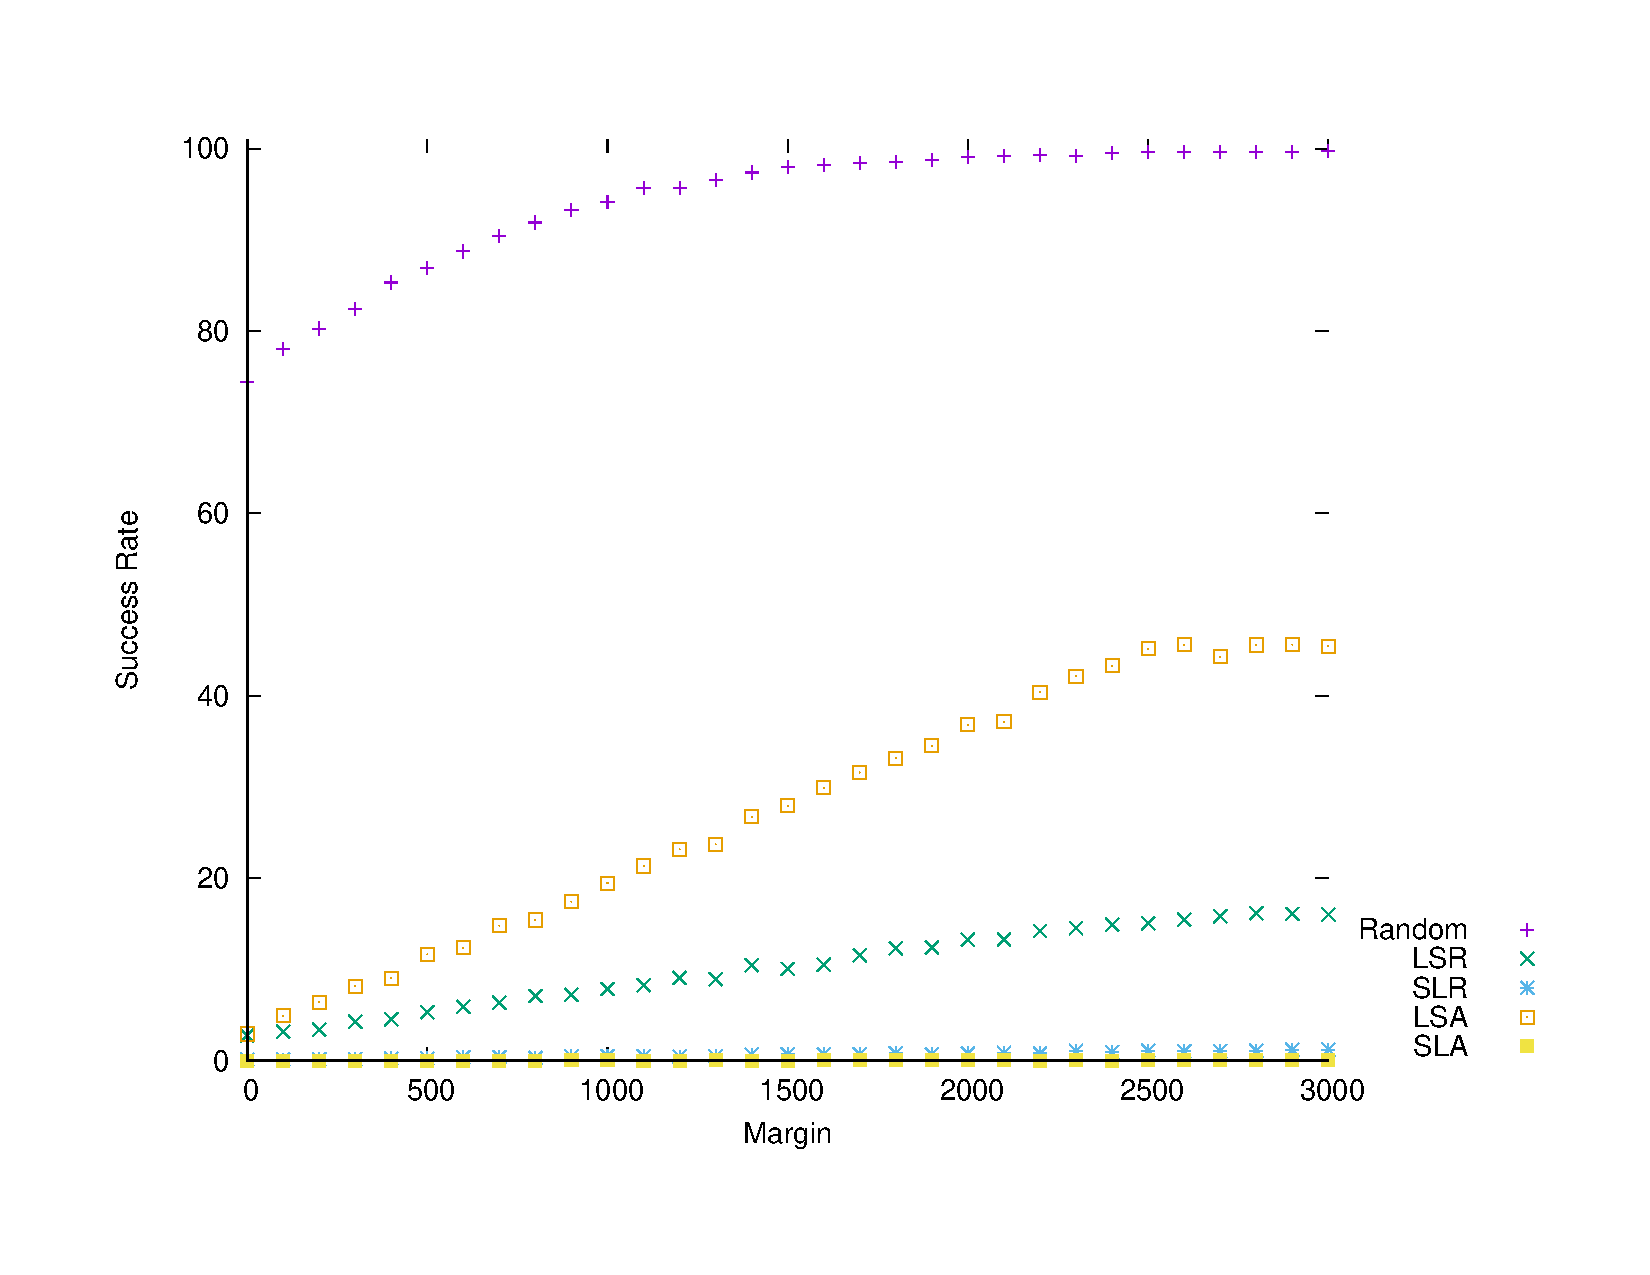
\includegraphics[width=6cm]{departs_gp_21000.pdf}

      \caption{Success rate of different orders with $P = 21000$}
      \end{minipage} \hfill
        \begin{minipage}[c]{6cm}
          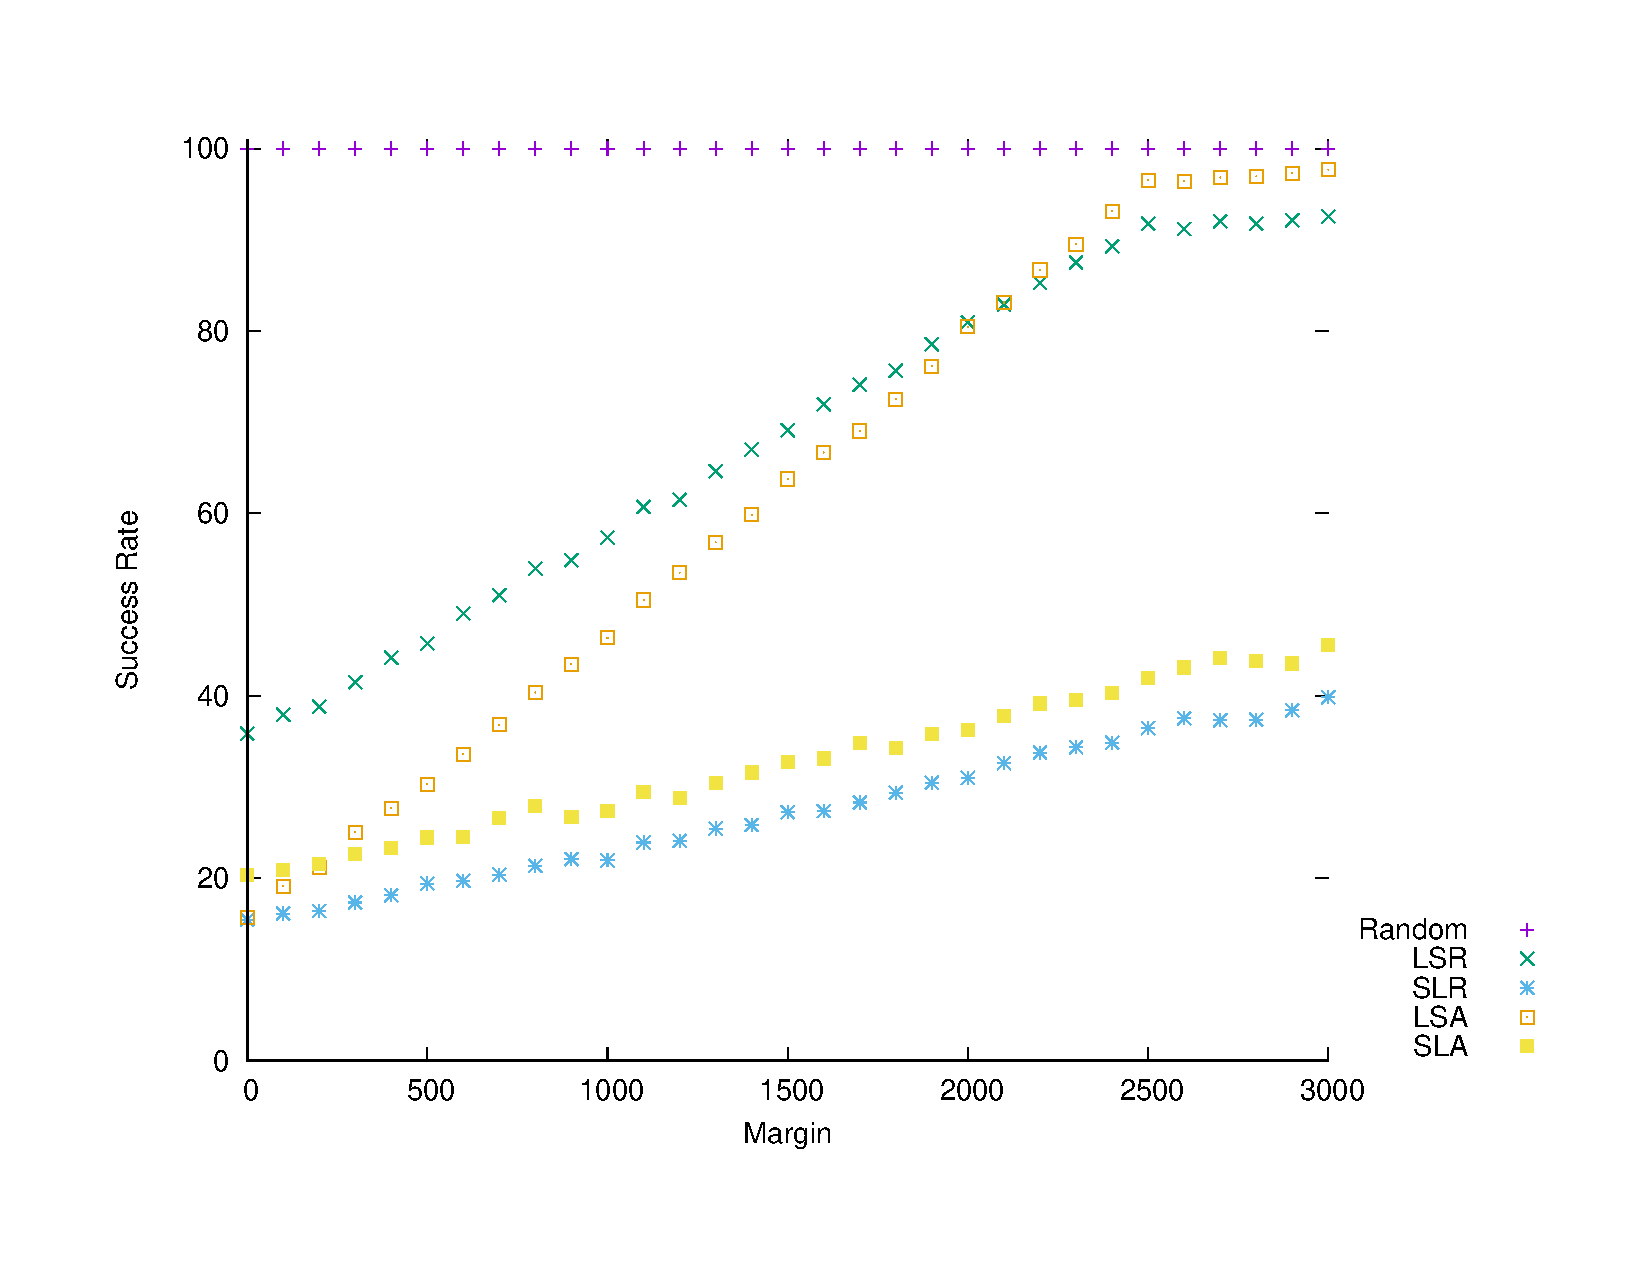
\includegraphics[width=6cm]{departs_gp_30000.pdf}
      \caption{Success rate of different orders with $P = 30000$}

            \end{minipage} \hfill
                  \label{fig:success30000}
     \end{figure}
     
     As expected, the  success rate is much better for large periods. According to our experiments, sending the messages from the shortest to the longest route or arc does not work well. It corresponds to the policy of Proposition~\ref{prop:SL} which does not work well when the routes are long as it is the case in these experiments. Sending from the longest to the shortest route or arc works better and it seems that sorting the routes according to the length of the last arc rather than the route is better, at least in a loaded network. 
     
     The random order is the best by far. When the load is not too high ($P = 30000$) there is always a solution with margin $0$.
     Note that, when disallowing waiting times, there were instances without solutions for these parameters (see Section~\ref{sec:exp_PAZL}), which justifies the interest of studying the PALL problem. We now want to compare the performances of the three different algorithms used in the second stage. Since GD already showed excellent results on mild loads, it is more interesting to focus on the behavior of the algorithms on high load. Moreover, we will use $1000$ random orders for the first stage as it gives the best results. The following experiment is realized on routed networks with $8$ routes, weights of the arcs drawn between $0$ and $20000$ and with a period of $21000$.  We represent the success rate with regards to the margin, for the three algorithms computed over $10000$ random star topologies. 
   

 
    \begin{figure} [H] 
       \begin{center}
      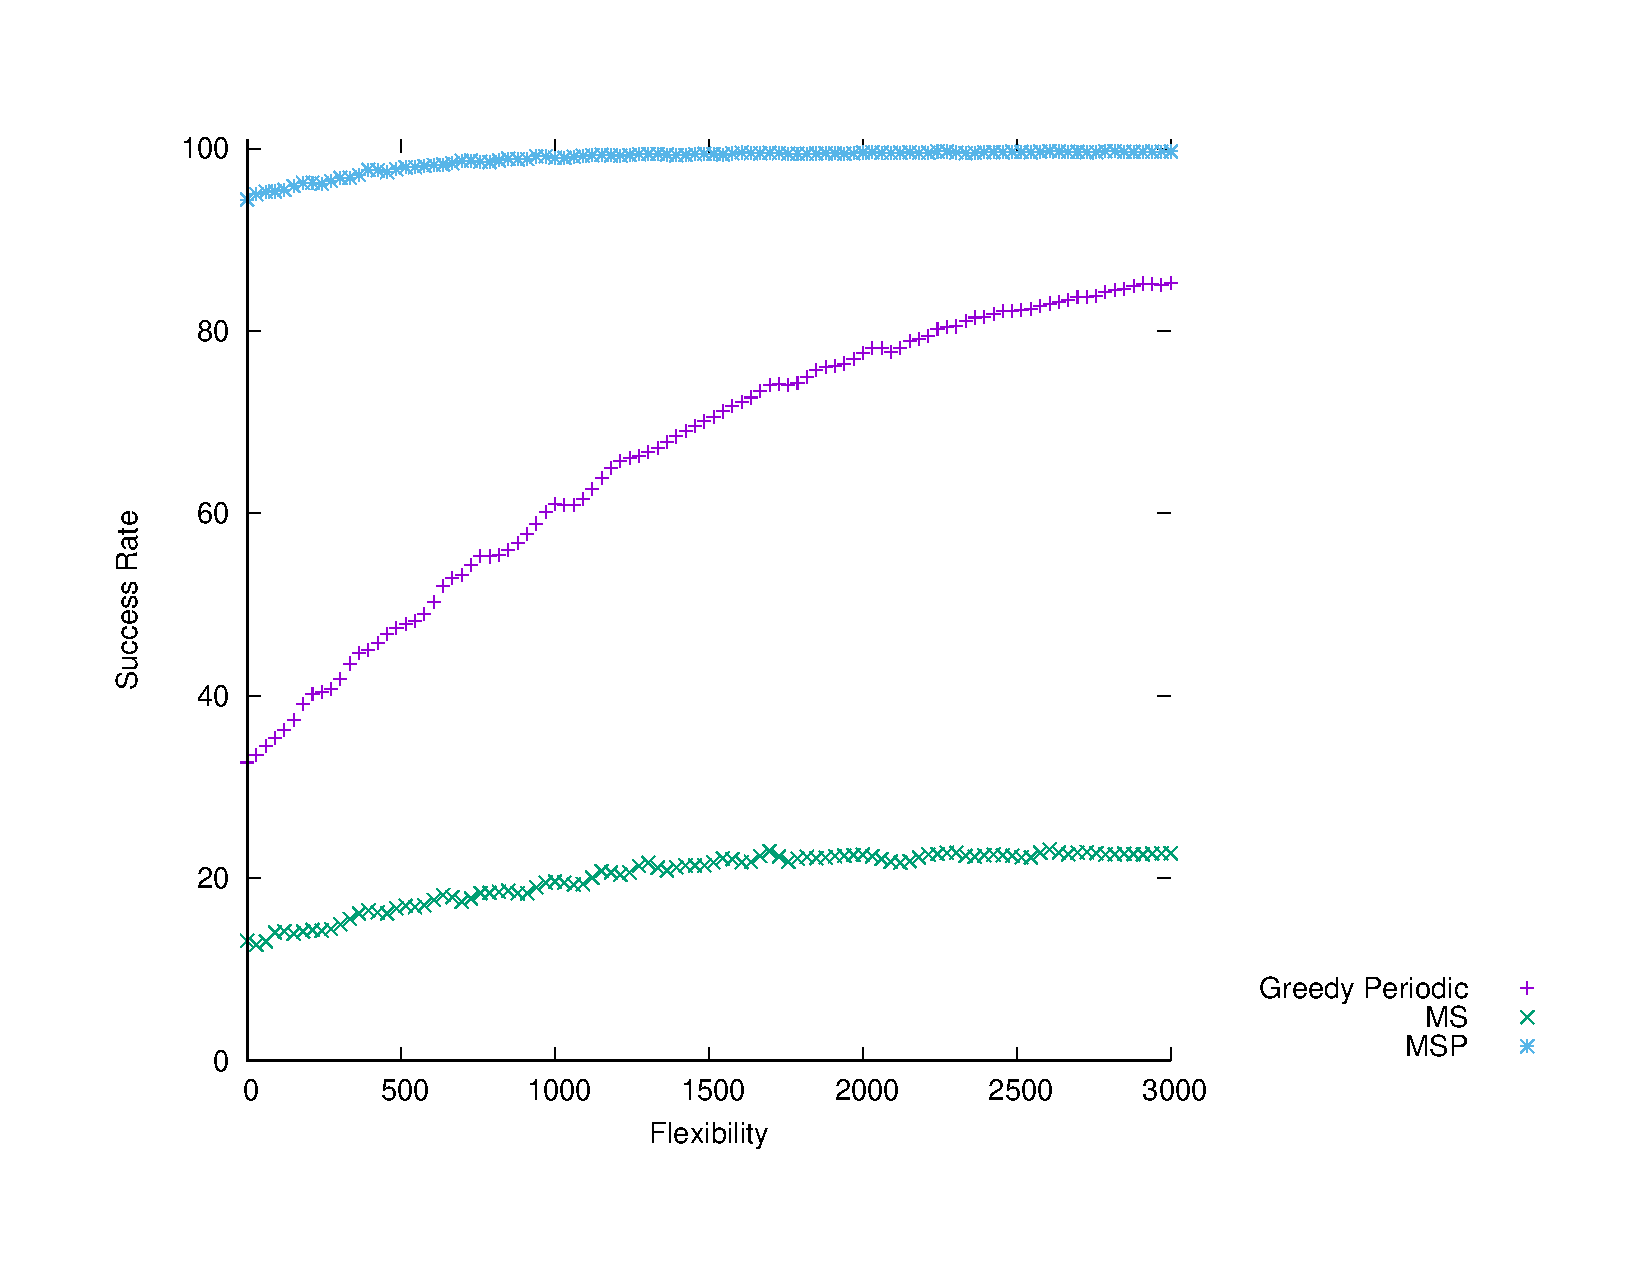
\includegraphics[scale=0.45]{retour_21000.pdf}
      \end{center}
      \caption{Success rate of GD, MLS and PMLS for $P = 21000$}
     \label{fig:success21000}
     \end{figure}
     
     The MLS algorithm performs poorly, worst than GD and PMLS, which shows that taking into account the periodicity is fundamental.
     The GD algorithms is close to $100\%$ success rate for margins larger than $1500$ while the PMLS algorithm finds a solution in more than $95\%$ of the experiments, even with a margin $0$. Therefore, for the worst possible constraints on load and margin, there are a few instances for which we do not find a solution. However, with a margin of $1000$, which corresponds to about $0.05$ms of additional delay with the chosen parameters, we always find a solution. 
     
    Remark that the random order corresponds to the best of $1000$ orders drawn uniformly which means that a computation can be up to $1000$ time slower than for a fixed order. The choice of the number of random orders drawn yields a trade-off between the computation time and the success rate. Up to now, we chose $1000$ random orders arbitrarily. We investigate the success rate of our algorithm with regards to the number of random orders drawn, a period of $21000$ and a margin $0$. The following tables presents the average success rate for each number of sending orders, on $1000$ instances, for GD and PMLS.

         \begin{figure}[H] 
       \begin{center}
   \begin{tabular}{|c|c|c|c|c|c|c|}
    \hline
    Number of random orders & $1$ & $10$ & $100$& $1 000$& $10 000$&$100 000$\\
    \hline
    Percentage of success of GD & $0.6$ &$7.1$&$33.4$&$76.4$&$90.0$&$90.0$\\
    \hline
    Percentage of success of PMLS & $41,1$ &$82,5$&$94,5$&$96,2$&$97,2$&$97,2$\\
    \hline
      \end{tabular}
      \end{center}
   \caption{Impact of the number of random sending orders}
     \end{figure}
     
First remark that we can improve our previous results by taking $10000$ random orders, which 
yields the best results for the two algorithms. The number of different orders is $7!= 5040$ since we have $8$ routes and the solutions are invariant up to a circular permutation of the order. Therefore instead of doing $10000$ random draws we could test every possible order in less time. However this method would not be practical with regard to the computation time for $n = 15$. On the other hand, remark that the success rate of PMLS is already high for $100$ random orders, which means it will work even better than the other methods when $n$ is larger and that the number of random orders drawn is critical.
     
     
     
     Now that we have found the best amongst the algorithms solving PALL, we need to compare its performances against the actual way to manage the messages in a network. The classical way to manage messages in the network is statistical multiplexing, where there is a FIFO buffer in each node of the network to deal with the collisions. The time at which the messages are sent in the network is not computed as in our approach, thus we fix the offsets of each route to some random value.
     Even if this policy seems to work in practice when the network is not too loaded, it does not give any guarantee on the latency. Remark that the process is not periodic, therefore we must measure the process time of each route over several periods if we want to compute its maximum. We choose to simulate it for $1000$ periods and we have observed that the process time usually stabilizes after $10$ periods. The margin is defined as the maximum process time, computed as explained, minus twice the size of the longest route. 
	    
     
     We draw $1000$ instances of a star topology with $8$ routes, with weights on the arcs drawn between $0$ and $20000$. Note that the results are almost the same when the arcs are small. We measure, for periods from $20000$ (network fully loaded), to $50000$ ($40 \%$ of load), the median, the first, and the third quartile of the margins computed in $1000$ simulations using FIFO buffer to resolve collisions.
     
      
    \begin{figure}[H] 

       \begin{center}
     % 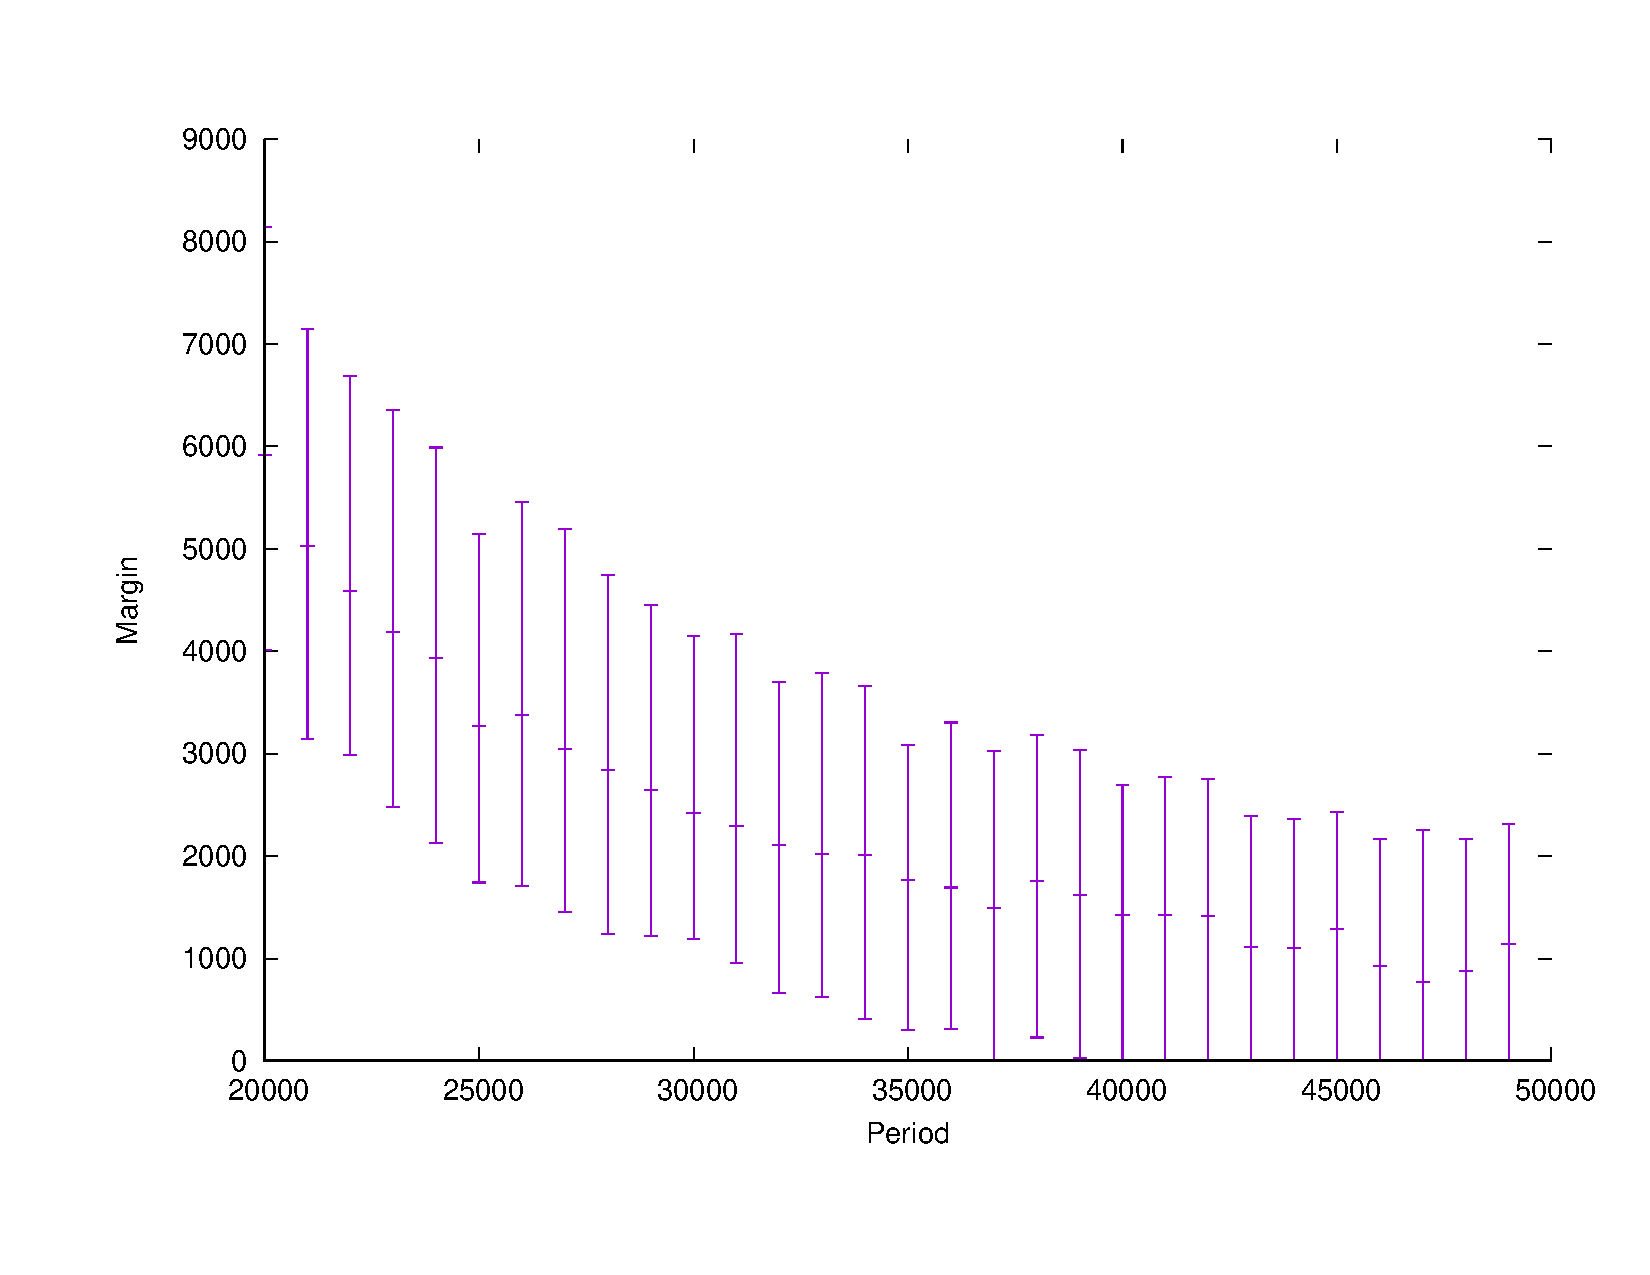
\includegraphics[scale=0.4]{stochastic.pdf}
       % GNUPLOT: LaTeX picture
\setlength{\unitlength}{0.240900pt}
\ifx\plotpoint\undefined\newsavebox{\plotpoint}\fi
\sbox{\plotpoint}{\rule[-0.200pt]{0.400pt}{0.400pt}}%
\begin{picture}(1500,900)(0,0)
\sbox{\plotpoint}{\rule[-0.200pt]{0.400pt}{0.400pt}}%
\put(171.0,131.0){\rule[-0.200pt]{4.818pt}{0.400pt}}
\put(151,131){\makebox(0,0)[r]{$0$}}
\put(1279.0,131.0){\rule[-0.200pt]{4.818pt}{0.400pt}}
\put(171.0,212.0){\rule[-0.200pt]{4.818pt}{0.400pt}}
\put(151,212){\makebox(0,0)[r]{$1000$}}
\put(1279.0,212.0){\rule[-0.200pt]{4.818pt}{0.400pt}}
\put(171.0,293.0){\rule[-0.200pt]{4.818pt}{0.400pt}}
\put(151,293){\makebox(0,0)[r]{$2000$}}
\put(1279.0,293.0){\rule[-0.200pt]{4.818pt}{0.400pt}}
\put(171.0,374.0){\rule[-0.200pt]{4.818pt}{0.400pt}}
\put(151,374){\makebox(0,0)[r]{$3000$}}
\put(1279.0,374.0){\rule[-0.200pt]{4.818pt}{0.400pt}}
\put(171.0,455.0){\rule[-0.200pt]{4.818pt}{0.400pt}}
\put(151,455){\makebox(0,0)[r]{$4000$}}
\put(1279.0,455.0){\rule[-0.200pt]{4.818pt}{0.400pt}}
\put(171.0,535.0){\rule[-0.200pt]{4.818pt}{0.400pt}}
\put(151,535){\makebox(0,0)[r]{$5000$}}
\put(1279.0,535.0){\rule[-0.200pt]{4.818pt}{0.400pt}}
\put(171.0,616.0){\rule[-0.200pt]{4.818pt}{0.400pt}}
\put(151,616){\makebox(0,0)[r]{$6000$}}
\put(1279.0,616.0){\rule[-0.200pt]{4.818pt}{0.400pt}}
\put(171.0,697.0){\rule[-0.200pt]{4.818pt}{0.400pt}}
\put(151,697){\makebox(0,0)[r]{$7000$}}
\put(1279.0,697.0){\rule[-0.200pt]{4.818pt}{0.400pt}}
\put(171.0,778.0){\rule[-0.200pt]{4.818pt}{0.400pt}}
\put(151,778){\makebox(0,0)[r]{$8000$}}
\put(1279.0,778.0){\rule[-0.200pt]{4.818pt}{0.400pt}}
\put(171.0,859.0){\rule[-0.200pt]{4.818pt}{0.400pt}}
\put(151,859){\makebox(0,0)[r]{$9000$}}
\put(1279.0,859.0){\rule[-0.200pt]{4.818pt}{0.400pt}}
\put(171.0,131.0){\rule[-0.200pt]{0.400pt}{4.818pt}}
\put(171,90){\makebox(0,0){$20000$}}
\put(171.0,839.0){\rule[-0.200pt]{0.400pt}{4.818pt}}
\put(359.0,131.0){\rule[-0.200pt]{0.400pt}{4.818pt}}
\put(359,90){\makebox(0,0){$25000$}}
\put(359.0,839.0){\rule[-0.200pt]{0.400pt}{4.818pt}}
\put(547.0,131.0){\rule[-0.200pt]{0.400pt}{4.818pt}}
\put(547,90){\makebox(0,0){$30000$}}
\put(547.0,839.0){\rule[-0.200pt]{0.400pt}{4.818pt}}
\put(735.0,131.0){\rule[-0.200pt]{0.400pt}{4.818pt}}
\put(735,90){\makebox(0,0){$35000$}}
\put(735.0,839.0){\rule[-0.200pt]{0.400pt}{4.818pt}}
\put(923.0,131.0){\rule[-0.200pt]{0.400pt}{4.818pt}}
\put(923,90){\makebox(0,0){$40000$}}
\put(923.0,839.0){\rule[-0.200pt]{0.400pt}{4.818pt}}
\put(1111.0,131.0){\rule[-0.200pt]{0.400pt}{4.818pt}}
\put(1111,90){\makebox(0,0){$45000$}}
\put(1111.0,839.0){\rule[-0.200pt]{0.400pt}{4.818pt}}
\put(1299.0,131.0){\rule[-0.200pt]{0.400pt}{4.818pt}}
\put(1299,90){\makebox(0,0){$50000$}}
\put(1299.0,839.0){\rule[-0.200pt]{0.400pt}{4.818pt}}
\put(171.0,131.0){\rule[-0.200pt]{0.400pt}{175.375pt}}
\put(171.0,131.0){\rule[-0.200pt]{271.735pt}{0.400pt}}
\put(30,495){\makebox(0,0){Needed Flexibility}}
\put(735,29){\makebox(0,0){Period}}
\put(171.0,455.0){\rule[-0.200pt]{0.400pt}{81.183pt}}
\put(171.0,455.0){\rule[-0.200pt]{2.409pt}{0.400pt}}
\put(171.0,792.0){\rule[-0.200pt]{2.409pt}{0.400pt}}
\put(209.0,412.0){\rule[-0.200pt]{0.400pt}{73.715pt}}
\put(199.0,412.0){\rule[-0.200pt]{4.818pt}{0.400pt}}
\put(199.0,718.0){\rule[-0.200pt]{4.818pt}{0.400pt}}
\put(246.0,353.0){\rule[-0.200pt]{0.400pt}{79.497pt}}
\put(236.0,353.0){\rule[-0.200pt]{4.818pt}{0.400pt}}
\put(236.0,683.0){\rule[-0.200pt]{4.818pt}{0.400pt}}
\put(284.0,336.0){\rule[-0.200pt]{0.400pt}{75.883pt}}
\put(274.0,336.0){\rule[-0.200pt]{4.818pt}{0.400pt}}
\put(274.0,651.0){\rule[-0.200pt]{4.818pt}{0.400pt}}
\put(321.0,306.0){\rule[-0.200pt]{0.400pt}{70.343pt}}
\put(311.0,306.0){\rule[-0.200pt]{4.818pt}{0.400pt}}
\put(311.0,598.0){\rule[-0.200pt]{4.818pt}{0.400pt}}
\put(359.0,297.0){\rule[-0.200pt]{0.400pt}{73.715pt}}
\put(349.0,297.0){\rule[-0.200pt]{4.818pt}{0.400pt}}
\put(349.0,603.0){\rule[-0.200pt]{4.818pt}{0.400pt}}
\put(397.0,270.0){\rule[-0.200pt]{0.400pt}{63.598pt}}
\put(387.0,270.0){\rule[-0.200pt]{4.818pt}{0.400pt}}
\put(387.0,534.0){\rule[-0.200pt]{4.818pt}{0.400pt}}
\put(434.0,269.0){\rule[-0.200pt]{0.400pt}{64.561pt}}
\put(424.0,269.0){\rule[-0.200pt]{4.818pt}{0.400pt}}
\put(424.0,537.0){\rule[-0.200pt]{4.818pt}{0.400pt}}
\put(472.0,238.0){\rule[-0.200pt]{0.400pt}{69.138pt}}
\put(462.0,238.0){\rule[-0.200pt]{4.818pt}{0.400pt}}
\put(462.0,525.0){\rule[-0.200pt]{4.818pt}{0.400pt}}
\put(509.0,226.0){\rule[-0.200pt]{0.400pt}{62.393pt}}
\put(499.0,226.0){\rule[-0.200pt]{4.818pt}{0.400pt}}
\put(499.0,485.0){\rule[-0.200pt]{4.818pt}{0.400pt}}
\put(547.0,222.0){\rule[-0.200pt]{0.400pt}{60.225pt}}
\put(537.0,222.0){\rule[-0.200pt]{4.818pt}{0.400pt}}
\put(537.0,472.0){\rule[-0.200pt]{4.818pt}{0.400pt}}
\put(585.0,195.0){\rule[-0.200pt]{0.400pt}{60.225pt}}
\put(575.0,195.0){\rule[-0.200pt]{4.818pt}{0.400pt}}
\put(575.0,445.0){\rule[-0.200pt]{4.818pt}{0.400pt}}
\put(622.0,185.0){\rule[-0.200pt]{0.400pt}{58.780pt}}
\put(612.0,185.0){\rule[-0.200pt]{4.818pt}{0.400pt}}
\put(612.0,429.0){\rule[-0.200pt]{4.818pt}{0.400pt}}
\put(660.0,178.0){\rule[-0.200pt]{0.400pt}{59.743pt}}
\put(650.0,178.0){\rule[-0.200pt]{4.818pt}{0.400pt}}
\put(650.0,426.0){\rule[-0.200pt]{4.818pt}{0.400pt}}
\put(697.0,188.0){\rule[-0.200pt]{0.400pt}{59.020pt}}
\put(687.0,188.0){\rule[-0.200pt]{4.818pt}{0.400pt}}
\put(687.0,433.0){\rule[-0.200pt]{4.818pt}{0.400pt}}
\put(735.0,152.0){\rule[-0.200pt]{0.400pt}{55.889pt}}
\put(725.0,152.0){\rule[-0.200pt]{4.818pt}{0.400pt}}
\put(725.0,384.0){\rule[-0.200pt]{4.818pt}{0.400pt}}
\put(773.0,146.0){\rule[-0.200pt]{0.400pt}{57.575pt}}
\put(763.0,146.0){\rule[-0.200pt]{4.818pt}{0.400pt}}
\put(763.0,385.0){\rule[-0.200pt]{4.818pt}{0.400pt}}
\put(810.0,146.0){\rule[-0.200pt]{0.400pt}{54.925pt}}
\put(800.0,146.0){\rule[-0.200pt]{4.818pt}{0.400pt}}
\put(800.0,374.0){\rule[-0.200pt]{4.818pt}{0.400pt}}
\put(848.0,143.0){\rule[-0.200pt]{0.400pt}{56.371pt}}
\put(838.0,143.0){\rule[-0.200pt]{4.818pt}{0.400pt}}
\put(838.0,377.0){\rule[-0.200pt]{4.818pt}{0.400pt}}
\put(885.0,140.0){\rule[-0.200pt]{0.400pt}{56.371pt}}
\put(875.0,140.0){\rule[-0.200pt]{4.818pt}{0.400pt}}
\put(875.0,374.0){\rule[-0.200pt]{4.818pt}{0.400pt}}
\put(923.0,133.0){\rule[-0.200pt]{0.400pt}{54.202pt}}
\put(913.0,133.0){\rule[-0.200pt]{4.818pt}{0.400pt}}
\put(913.0,358.0){\rule[-0.200pt]{4.818pt}{0.400pt}}
\put(961.0,131.0){\rule[-0.200pt]{0.400pt}{55.166pt}}
\put(951.0,131.0){\rule[-0.200pt]{4.818pt}{0.400pt}}
\put(951.0,360.0){\rule[-0.200pt]{4.818pt}{0.400pt}}
\put(998.0,131.0){\rule[-0.200pt]{0.400pt}{49.384pt}}
\put(988.0,131.0){\rule[-0.200pt]{4.818pt}{0.400pt}}
\put(988.0,336.0){\rule[-0.200pt]{4.818pt}{0.400pt}}
\put(1036.0,131.0){\rule[-0.200pt]{0.400pt}{48.180pt}}
\put(1026.0,131.0){\rule[-0.200pt]{4.818pt}{0.400pt}}
\put(1026.0,331.0){\rule[-0.200pt]{4.818pt}{0.400pt}}
\put(1073.0,131.0){\rule[-0.200pt]{0.400pt}{47.216pt}}
\put(1063.0,131.0){\rule[-0.200pt]{4.818pt}{0.400pt}}
\put(1063.0,327.0){\rule[-0.200pt]{4.818pt}{0.400pt}}
\put(1111.0,131.0){\rule[-0.200pt]{0.400pt}{46.975pt}}
\put(1101.0,131.0){\rule[-0.200pt]{4.818pt}{0.400pt}}
\put(1101.0,326.0){\rule[-0.200pt]{4.818pt}{0.400pt}}
\put(1149.0,131.0){\rule[-0.200pt]{0.400pt}{45.048pt}}
\put(1139.0,131.0){\rule[-0.200pt]{4.818pt}{0.400pt}}
\put(1139.0,318.0){\rule[-0.200pt]{4.818pt}{0.400pt}}
\put(1186.0,131.0){\rule[-0.200pt]{0.400pt}{46.494pt}}
\put(1176.0,131.0){\rule[-0.200pt]{4.818pt}{0.400pt}}
\put(1176.0,324.0){\rule[-0.200pt]{4.818pt}{0.400pt}}
\put(1224.0,131.0){\rule[-0.200pt]{0.400pt}{45.048pt}}
\put(1214.0,131.0){\rule[-0.200pt]{4.818pt}{0.400pt}}
\put(1214.0,318.0){\rule[-0.200pt]{4.818pt}{0.400pt}}
\put(1261.0,131.0){\rule[-0.200pt]{0.400pt}{41.194pt}}
\put(1251.0,131.0){\rule[-0.200pt]{4.818pt}{0.400pt}}
\put(171,608){\makebox(0,0){$+$}}
\put(209,562){\makebox(0,0){$+$}}
\put(246,503){\makebox(0,0){$+$}}
\put(284,479){\makebox(0,0){$+$}}
\put(321,431){\makebox(0,0){$+$}}
\put(359,429){\makebox(0,0){$+$}}
\put(397,390){\makebox(0,0){$+$}}
\put(434,382){\makebox(0,0){$+$}}
\put(472,367){\makebox(0,0){$+$}}
\put(509,340){\makebox(0,0){$+$}}
\put(547,327){\makebox(0,0){$+$}}
\put(585,317){\makebox(0,0){$+$}}
\put(622,307){\makebox(0,0){$+$}}
\put(660,302){\makebox(0,0){$+$}}
\put(697,300){\makebox(0,0){$+$}}
\put(735,278){\makebox(0,0){$+$}}
\put(773,273){\makebox(0,0){$+$}}
\put(810,268){\makebox(0,0){$+$}}
\put(848,267){\makebox(0,0){$+$}}
\put(885,254){\makebox(0,0){$+$}}
\put(923,248){\makebox(0,0){$+$}}
\put(961,259){\makebox(0,0){$+$}}
\put(998,234){\makebox(0,0){$+$}}
\put(1036,234){\makebox(0,0){$+$}}
\put(1073,232){\makebox(0,0){$+$}}
\put(1111,228){\makebox(0,0){$+$}}
\put(1149,216){\makebox(0,0){$+$}}
\put(1186,212){\makebox(0,0){$+$}}
\put(1224,227){\makebox(0,0){$+$}}
\put(1261,203){\makebox(0,0){$+$}}
\put(1251.0,302.0){\rule[-0.200pt]{4.818pt}{0.400pt}}
\put(171.0,131.0){\rule[-0.200pt]{0.400pt}{175.375pt}}
\put(171.0,131.0){\rule[-0.200pt]{271.735pt}{0.400pt}}
\end{picture}

      \end{center}
      \caption{Needed margin with respect to the period for a stochastic policy}
      \label{fig:sto}
     \end{figure}
     
     We have also computed the minimum margin needed by PMLS to find a solution but we have not represented it in Figure~\ref{fig:sto} since even the third quartile was always at $0$ for a period of $20000$.
     There is around $20\%$ of the instances for which the margin is larger than $0$ for $P=20000$ and $7\%$
     for $P = 21000$. For the instances with a margin larger than $0$, the margin is on average $400$.
     
     The simulations show clearly that the stochastic policy does not ensure a minimal latency. As we can see in Fig~\ref{fig:sto}), the more the network is loaded, the higher the latency is. When the network is highly loaded,
     we have instances with a margin of about $10000$ which corresponds to half the period, that is $0.5$ms. 
     Even when the network is lightly loaded, a quarter of the instances have a margin of more than $2000$
     which is more than what PMLS finds for the worst instance and a network fully loaded ! 
     We feel that it strongly justifies the use of a deterministic sending scheme for latency critical applications such as our C-RAN motivating problem.
     
    
    \paragraph*{Future works}
   
   We plan to generalize our study of the PALL problem to other topologies,
   such as trees, cycles or bounded treewidth graphs. 
   We would like to design FPT algorithms in the number of routes for PAZL and PALL on the star topology, eventually by relaxing the constraint on the maximal process time into an constraint on the average process time, which seems much more tractable. 
   
   We could also study variation of our problem. Instead of minimizing the maximum process time, we could try to minimize
   the sum of the waiting time, a linear objective which could make linear programming useful.
   Moreover we could allow preemption, that is the messages are allowed to be cut into pieces, which would certainly change the complexity of the problem. 
   Finally, the routes may not be fixed but chosen in the graph to minimize the maximum process time, which would make the problem even more difficult (maybe $\Pi_2$-complete instead of $\NP$-complete). 

   
  \paragraph*{Acknowledgments} The authors thanks Christian Cadere and David Auger for the friendly discussions
  they had on the subject and their insightful remarks. 

\bibliographystyle{ieeetr}
\bibliography{Sources}

\end{document}
